%!TEX encoding = UTF-8 Unicode
%!TEX program = latexmk

\documentclass[master,professional]{ustcthesis}
% doctor|master|bachelor [academic|professional] [chinese|english] [print|pdf]
% [super|numebers|authoryear]

\title{软件定义网络轻量级sketch测量与分布式部署研究}
\author{于希文}
\major{软件工程}
\supervisor{徐宏力}
% \date{二〇一七年五月一日} % 注释掉则为今日
\professionaltype{专业学位类型}
% \secretlevel{秘密}        % 绝密|机密|秘密,注释本行则不保密
% \secretyear{20}           % 保密年限

\entitle{Lightweight Sketch Measurement and Distributed Deployment for Software-Defined Networks}
\enauthor{Xiwen Yu}
\enmajor{Software Engineering}
\ensupervisor{Hongli Xu}
% \endate{May 1, 2017}      % Today if commented
% \enprofessionaltype{Professional degree type}
% \ensecretlevel{Secret}    % Top secret|Highly secret|Secret

% 额外的宏包和配置写进 ustcthesis-extra.sty
\usepackage{ustcthesis-extra}



\begin{document}

% 研究生论文:
%   封面,原创性声明和授权使用声明
%   frontmatter: 摘要,目录,[图、表清单],[符号说明]
%   mainmatter: 正文章节,参考文献
%   appendix: 附录
%   backmatter: 致谢,已发表论文列表
%
% 本科生论文:
%   封面
%   frontmatter: 致谢,目录,摘要
%   mainmatter: 正文章节,参考文献
%   appendix: 附录

\maketitle
\makestatement

\frontmatter
\begin{abstract}
软件定义网络(SDN)是新一代的网络架构。
通过将控制层与数据层分离,SDN能够对网络进行细粒度优化,从而提高资源利用效率,适应迅猛发展的互联网业务。
在SDN中,流量统计信息对网络优化十分重要,如重路由、攻击检测等。
然而,SDN交换机中的部分硬件资源十分有限,如TCAM、SRAM的存储资源以及CPU的计算资源。
随着网络中流量的增加,传统的基于流表的测量方法和基于采样的测量方法由于受这些资源的限制,无法继续保证测量精度。
因此,基于sketch的测量方法走进视野。

Sketch可以利用很少的存储空间来找出特定种类的流,以及它们的流量统计信息。
而网络中的最大的若干条流(top-$k$)的流量统计信息是最为重要的,因此能够测量top-$k$的sketch受到了更多关注。
然而,根据分析,当网络负载较大的时候,现有的若干种sketch会占用过多的CPU计算资源。
过多消耗CPU计算资源有可能会影响交换机的基础功能,如流表的插入和修改等。
为了解决CPU计算资源不足的问题,我们从数据平面和控制平面分别入手。
在数据平面,我们可以通过设计更加轻便快速的sketch来降低计算负载。
在控制平面,我们则可以通过分布式部署的方法,让交换机只测量一部分数据包,减少不同交换机重复测量同一条流的情况,从而在不牺牲测量精度的情况下降低计算负载。

% 在网络中流量不断增大的情况下,让交换机测量所有经过的数据包势必会加大计算负载并导致测量的冗余。


本文的第一部分着眼于数据平面,提出了一种基于哈希碰撞的新型轻量级sketch,命名为CountMax。
它能够在网络中找出top-$k$的流ID,并测量这些大流的流量。
和已有的sketch相比,CountMax在理论上拥有更低的时间复杂度,以及有界的测量精度。
我们还讨论了使用CountMax进行流重路由,以及进一步降低计算负载的CountMax的协作式部署。
实验结果显示,CountMax的测量精度和已有的sketch持平或者略高,计算负载比已有的sketch减少了约50\%。

本文的第二部分聚焦于控制平面,讨论了流量测量在网络中的分布式部署问题。
通过问题的建模和形式化,我们提出了一个基于贪心法实现最大流统计覆盖的算法,称为GMSC。
控制器使用GMSC为每个交换机生成规则,交换机上只需对符合规则的流进行测量。
我们在理论上证明了GMSC算法的有效性。并使用仿真模拟测试了GMSC+CountMax的性能。
测试结果显示,与协作式部署相比,使用GMSC的部署方案可以提升约20\%的测量精度,同时将交换机负载减少约30\%。
最后,本文还在Open vSwitch平台上实现了CountMax和GMSC,证明了本文研究成果的可行性。

\keywords{软件定义网络;流量测量;Sketch;优化算法}
\end{abstract}

\begin{enabstract}
By separating the control plane and the data plane, an SDN can provide fine-grained management and optimize the network resource utilization. 
Statistics information is of vital importance for different applications in SDNs, such as traffic engineering, flow rerouting, and attack detection. 
Since some resources, e.g., TCAM, SRAM and computing capacity, are often limited on SDN switches, traffic measurements based on flow tables or sampling become infeasible. 
Sketches can find out flows of specified type along with their traffic statistics using little memory. 
Although many efficient sketches have been designed, our analysis shows that existing sketch-based measurement solutions may suffer from severe computing overhead on switches especially under high traffic load, which significantly interferes with switch's basic functions, such as flow rule setup and modification. 
%Moreover, as the network traffic keeps growing, measuring every packet in every switch brings more redundant computing overhead.
In order to reduce the computing overhead, we can introduce a faster sketch to data plane, and use distributed deployment in the control plane to decrease the redundancies of measurement.

In the first part of the paper, we focus on the data plane and present CountMax, a lightweight sketch for traffic measurement, which can find out the top-$k$ elephant flows and their traffic sizes. 
Compared with existing sketches, CountMax has lower time complexity in theory and bounded measurement error. 
We also discuss CountMax-based flow rerouting and cooperative deployment of CountMax. 
According to the results of testbed experiments and simulations, compared with existing sketches, CountMax reduces computing overhead by about 1/2 and has the same or lower estimation error.

In the second part, we introduce the traffic measurement deployment problem and propose a greedy algorithm of the Maximum Statistics Coverage problem, named GMSC, and analyze its approximation performance. 
GMSC generates rules for every switch, so that each switch only needs to measure flows that meets the rules.
As the simulations show, deploying sketches using GMSC can further reduce the computing overhead per switch by about 30\%, and achieve higher measurement accuracy, by about 20\%. 
At last, we implement CountMax and GMSC in Open vSwitch to prove the feasibility of our work.

\enkeywords{Software Defined Networks; Traffic Measurement; Sketch; Optimization Algorithm}
\end{enabstract}
\tableofcontents
% \listoffigures
% \listoftables
% \listofalgorithms
% %!TEX root = ../main.tex

\begin{notation}

\centering
\begin{tabular}{rl}
$\ln x$ & natural logarithm $\log_ex$ \\
$\log x$ & common logarithm $\log_{10}x$ \\
$x\ \mathrm{mod}\ y$ & remainder \\
\end{tabular}

\end{notation}


\mainmatter
\chapter{绪论}
本章首先介绍了软件定义网络的基础背景,随后介绍SDN当中的流量测量,以及现有的流量测量方式的局限,最后引出本文的研究内容。
\section{软件定义网络(SDN)}
随着互联网技术的高速发展,如今的互联网有着数据流量大、拓扑结构复杂、业务类型繁多的特点。
传统的网络结构体系在面对如今的互联网时逐渐显得力不从心,主要体现在维护困难、效率低、扩展性和兼容性不佳、安全性不足等。
传统网络中的每个路由器各自为战,通过一定的路由协议互相传递拓扑和链路信息,并独立维护一份信息。
这种方式的优点在于这样组成的网络是自组织的,在协议兼容的前提下可以轻易地向网络中加入结点,路由设施会自动完成路由表的更新。
而缺点在于,每个路由器所保存的拓扑信息和链路信息都是不完整的,很容易出现不同的源到同一目的的流量,由于路由算法汇聚到一起的现象,从而造成链路拥塞\cite{vissicchio2015central};
另一个问题是当设备或链路因为故障、维护、升级等原因出现变化,依靠路由协议传播变化信息耗时长且不稳定,可能会造成服务中断\cite{xu2018achieving}。
追根溯源,这一问题的根源来自于传统网络结构的前身,1969年由美国国防部提出的APRANet。
由于冷战时期的特殊时代背景以及APRANet的军方背景,最初的设计着重于网络中部分结点遭到破坏后,其余部分的自我恢复能力。
而在50年后的今天,互联网早已渗透进了人们生活的每个角落,民用和商用网络无需担心战火的破坏,这样的设计反而成为了限制网络性能的累赘。

在这样的背景下,软件定义网络(Software-Defined Network, SDN)\cite{mckeown2008openflow}应运而生。
SDN的核心思想是将网络中的控制系统与数据转发系统分离开来,形成控制平面和数据平面两个平行的结构。
其中控制平面由一个或多个控制器组成,数据平面由众多交换机组成。控制器与交换机之间通过控制协议交流,其中最为广泛使用的是OpenFlow协议。
通过OpenFlow协议,SDN中的控制器可以得知整个网络的拓扑和统计信息,由此在全局层面维护整个网络。
SDN交换机与传统网络中的路由器存在较大的区别。第一,SDN交换机无需维护网络拓扑和链路信息。
SDN交换机中存放着一张或多张流表,每个数据包根据流表进行匹配并采取对应的操作。
当数据包无法匹配所有流表中的任何表项时,交换机会将该数据包上传给控制器,由控制器为其分配操作,并将这一规则转换为流表项下发至所有相关的交换机。
第二,SDN交换机可以对流进行精确匹配。传统路由器中的路由表是根据目的地址进行匹配的,而SDN中的流表项可以匹配各种各样的协议字段。
如TCP\footnote{Transmission Control Protocol,传输控制协议}/UDP\footnote{User Datagram Protocol,用户数据报协议}的源/目的端口、
MPLS\footnote{Multi-Protocol Label Switching,多协议标签交换}标记\cite{davie2000mpls}、
ICMP\footnote{Internet Control Message Protocol,Internet控制报文协议}报文类型、ARP\footnote{Address Resolution Protocol,地址解析协议}操作类型(opCode)等都可以作为SDN流表项中的匹配域。
精密的匹配方式使得SDN可以实现对流的细粒度管理\cite{xu2017joint}。

通过使用OpenFlow与交换机通信,SDN的控制平面可以获取整个网络的几乎所有信息。
依靠这些信息,SDN可以实现对网络的全局优化。控制器与交换机之间的从属关系也使得网络维护人员能够更方便地对交换机的各种行为进行管理。
这些特点使得SDN相比传统网络可以更加方便的部署各种应用,如服务链(Service Function Chain)\cite{halpern2015service}、QoS\footnote{Quality of Service,服务质量}\cite{akella2014quality}等。

特别值得一提的是网络功能虚拟化(Network Function Virtualization, NFV)。
传统的网络通常会部署专门的设备来对网络数据进行处理,如防火墙、IPS\footnote{Intrusion Prevention System,入侵防御系统}等。
使用专用物理设备处理数据的缺点在于难以维护。设备升级和维护往往需要暂时断开网络连接,影响服务的持续性。
NFV的核心思想是使用一系列的通用设备代替这些专用设备,使用软件规则确定数据包要被哪些功能处理。
尽管NFV和SDN之间不存在依赖关系,但是NFV与SDN的设计是互补的。
SDN可以轻易地实现NFV中的规则匹配、集中管理的功能,同时SDN也可以吸收NFV的思想,将控制器、交换机虚拟化,提供更灵活的网络服务。
因而,在许多研究和应用当中,NFV和SDN是相伴相生的。

\begin{figure}[ht]
	\centering
	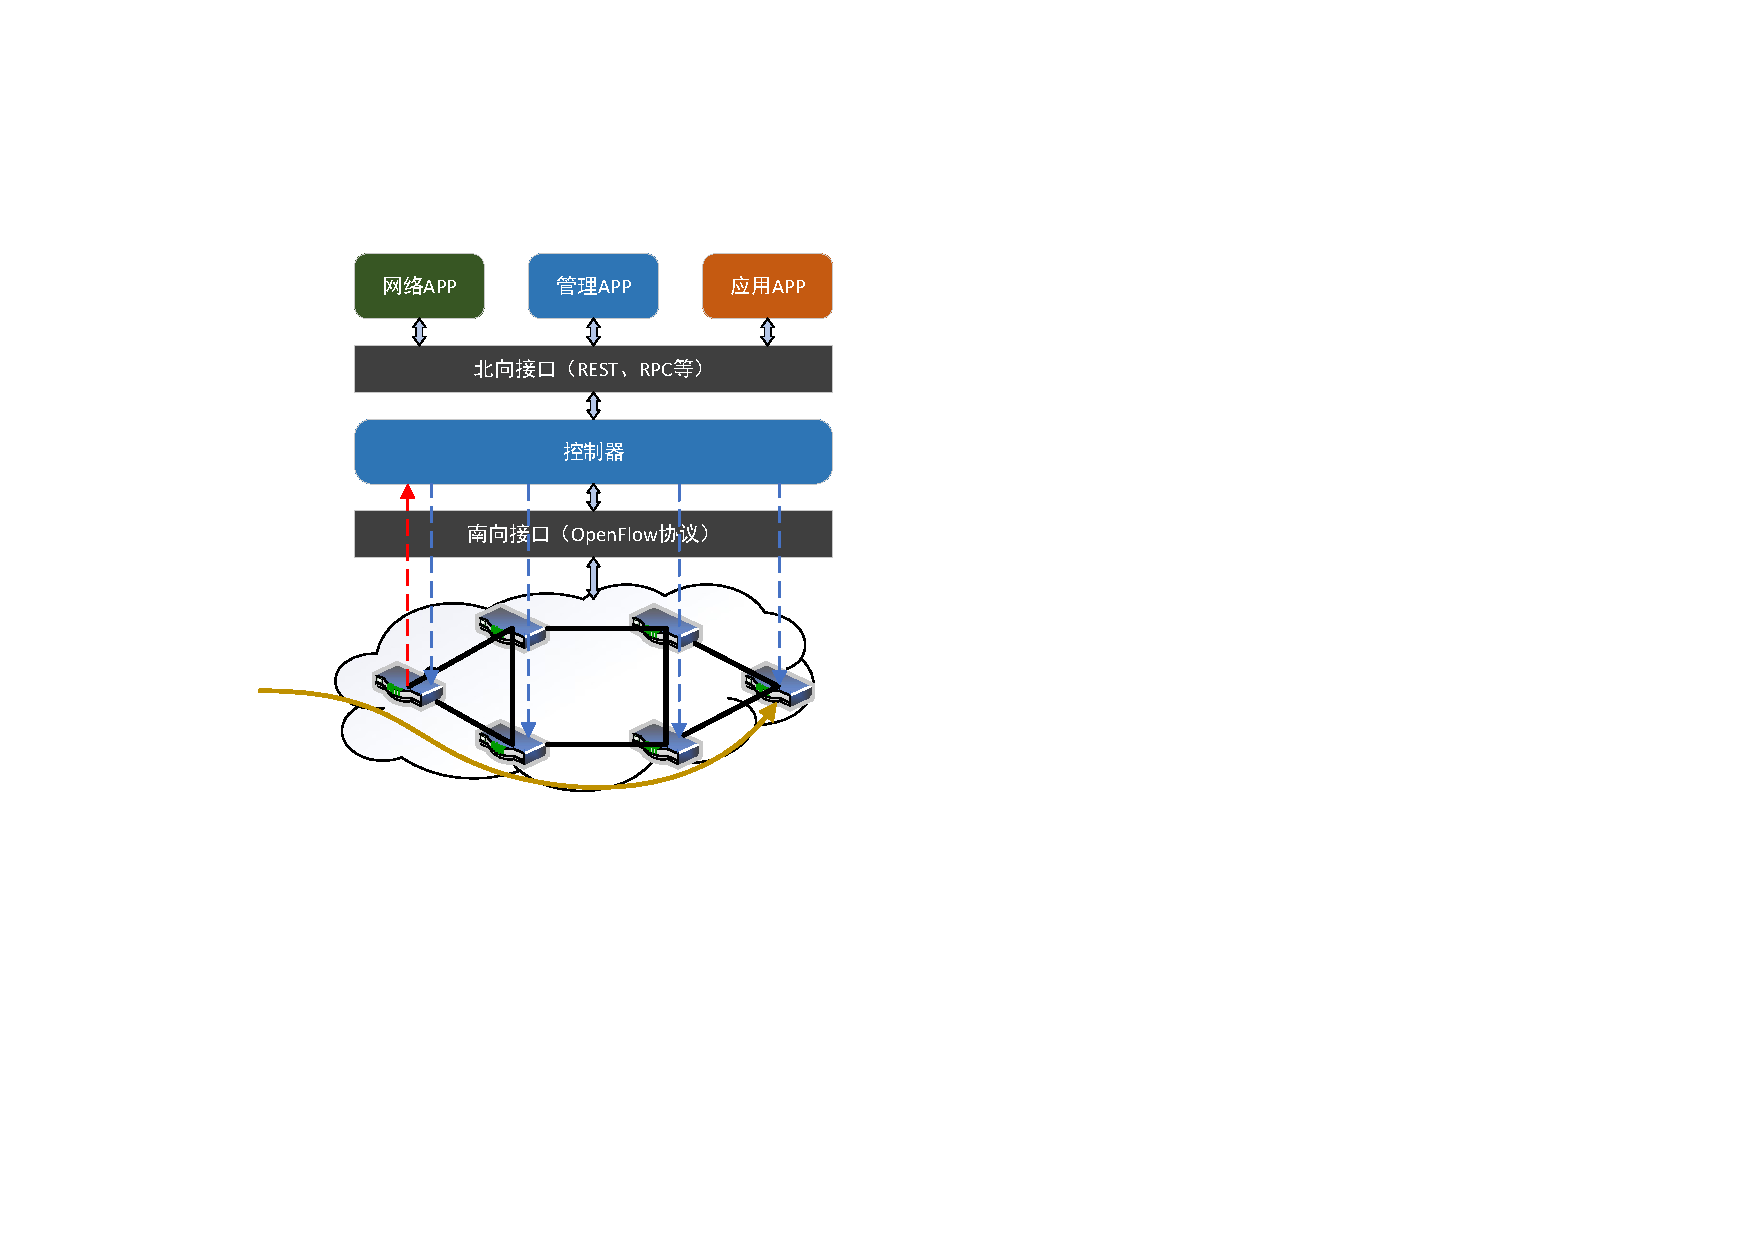
\includegraphics[width=0.8\linewidth]{fig/sdn.pdf}
	\caption{SDN网络结构}\label{fig:sdn}
\end{figure}

图\ref{fig:sdn}简要描绘了SDN的结构。图中的虚线表示了SDN中流表建立的过程。
最左侧的交换机收到一个无法匹配的数据包,通过红色虚线将其上传到控制器,控制器计算出路径后通过蓝色虚线将流表项下发给沿途的交换机,从而在网络中建立了一条新流。

截至目前,SDN已经在许多大型数据中心中得到了应用,包括Microsoft Azure、AWS、Google、阿里云等。
和其它的网络环境相比,数据中心网络有着流量大、可用性要求高、设备集中、统一管理的特点。
其中前两个特点是传统网络难以应付的,而SDN更容易实现的,构成了对SDN需求。
而后两个特点则大幅减少了SDN的部署阻力。

除数据中心之外,SDN近年来也开始在更多的领域走向实用。
在即将投入使用的5G通信中,SDN扮演着重要的角色\cite{zhang2017network};
包括中国电信在内的传统电信服务提供商也开始尝试将SDN用于民用;
思科、华为、IBM、惠普等等网络设备提供方也纷纷推出了基于SDN的产品。
我们可以说,SDN在未来将会成为主流的网络结构。

\section{SDN中的流量测量}\label{sec:measurement}
为了实现网络的优化,流量统计信息对SDN是至关重要的。流的路由、QoS、入侵检测等应用都十分依赖于流的流量统计信息。
然而,SDN交换机的硬件资源限制了流量统计的能力,主要体现在以下三种重要的硬件资源上。
\textbf{第一种资源是三态内容寻址存储器(Ternary Content Addressable Memory, TCAM)。}
与普通的根据地址寻址的RAM不同,TCAM根据匹配字段的内容进行寻址,因而可以极快地完成查找和匹配的任务。
由于交换机要频繁地对流表进行匹配,因而往往使用TCAM来存储流表。
然而,TCAM的造价十分昂贵,并且非常耗电。受成本所限,交换机中配备的TCAM容量往往十分有限,这也导致交换机中的流表项条目数受限。
例如HP 5406zl型号交换机只能容纳1500条流表项\cite{curtis2011devoflow}。
\textbf{第二种资源是静态随机存取存储器(Static Random-Access Memory,SRAM)。}交换机中的SRAM扮演着主存储器的角色。受成本因素影响,中低端交换机的SRAM大小往往也很有限,甚至使用更加缓慢的DRAM。
如Juniper入门款交换机仅仅有32MB的SRAM空间\cite{ResourceMonitoring},并且这仅有的SRAM上还承载着包括防火墙、路由控制在内的多种功能。
\textbf{第三种资源是CPU的计算资源。}SDN交换机最主要的功能是转发数据包,因此绝大多数的交换机都配备有专门的芯片用来转发数据包,以获得更高的吞吐率。
SDN交换机中的CPU则负责转发数据包之外的计算任务,因此其计算能力通常不高。市面上一些交换机的CPU仍在使用较为落后的MIPS指令集,主频甚至不足1GHz\cite{wang2014scotch}。

在SDN当中进行流量统计,目前有三种主流方法。第一种方法是使用交换机中的TCAM流表来进行统计。根据OpenFlow协议\cite{pfaff2012openflow},每个流表项当中都有一个字段用来统计符合该流表项的总流量。
然而如前所述,TCAM的容量限制了流表项的条目数。即使是比较高端的Boradcom Trident2型号,其流表最多也只支持1.6万个条目\cite{cohen2014effect}。
而数据中心当中的流的数量动辄上百万\cite{kandula2009nature},1.6万个条目显然远远不够。
当网络中的流数超出流表上限时,常用的解决方法是将多条流通过规则整合的方式整合到一个流表项中\cite{zhao2018joint},如只匹配部分字段或使用掩码,或者使用默认路径。
在这种情况下,流表项中统计的是符合该规则的所有流的流量,从而导致无法得知其中单个流的流量。

第二种方法是通过采样的方式进行统计,比如当前大多数交换机所支持的NetFlow\cite{estan2004building}或sFlow\cite{phaal2004sflow}解决方案。
然而,采样统计的测量精度常常不尽如人意\cite{yu2013software}\cite{li2016flowradar}。
提高采样统计的精度的最直接方法就是提高采样频率,但提高采样频率意味着消耗更多的计算和内存资源,从而影响此方案在有着更多流量的网络中的可伸缩性。

第三种方法是使用称为“sketch”的数据结构进行流量统计。
在实际应用场景中,我们往往并不需要得知所有流的流量统计信息,而只关心其中一部分特殊流的信息。
通过特殊的算法,sketch可以利用很少的内存空间来统计所有数据包,并且只留下关注的信息。
目前已经有很多种不同的sketch被设计出来,分别适用于不同的使用场景,并在测量精确度和资源占用中取得平衡\cite{KXW06}\cite{li2012per}\cite{estan2002new}。
然而,根据第\ref{chap:sketch}章中的研究,现有的基于sketch的流量测量方案大多数都面临着占用计算资源过多的问题。

值得注意的是,目前为止的绝大多数流量测量方案都只关注数据平面的单个交换机,却很少考虑整个网络中的联合优化。
例如,现有的基于流表的统计方式中,每个交换机都会统计经过它的所有流。对于一条经过多个交换机的流而言,这种方案会带来非常大的冗余。
不过,由于交换机使用速度极快的TCAM存储流表,且所有数据包都必须匹配流表,流量统计只需要“顺便”累加一个计数器,因而这种冗余对性能的影响微乎其微。

然而当引入sketch之后,流量测量冗余的问题就凸显出来了。
因为sketch一般存放在SRAM中,且存储器的速度往往慢于CPU,CPU不可避免地要对读写操作进行等待。
另外,每个数据包都要进行相对复杂的算法处理,因此sketch的计算负载不可能无限地降低,最终导致处理速度和流表相比始终会有较大差距。
因而必须考虑测量的冗余性所带来的额外计算负载。
如果我们不再将视线聚焦于单个交换机,而是着眼于整个网络,那么则可以通过流量测量的分布式部署来对网络中的流量测量进行整体优化。

\section{文章结构}
根据第\ref{sec:measurement}节的介绍,本文的研究目标主要有以下三点:

第一点是设计一种能够测量大流流量的高效的sketch。
对于SDN中的很多应用,最为关心的往往是如何获得网络中流量最大的若干条流的流量(也被称为top-$k$问题)。
例如,在实际场景中,控制器经常会向交换机部署默认路径以提升新流的响应速度,当许多流携带着大量流量同时经由默认路径转发时,网络中有可能会出现拥堵。
解决此问题的一种方案是,从这些通过默认路径的流当中找出其中流量较大的一些流,对它们进行重路由,从而实现更好的负载均衡。
因此,在交换机的层面,得知大流的较为准确的流量统计数据是非常重要的。
%其中设计的重点在于“高效”,也就是在不牺牲太多测量精度的前提下,尽量地减少sketch本身的计算负载。
如前文所述,由于交换机的CPU性能较弱,且还需要负责执行OpenFlow控制协议以及其它维持交换机运行的必要功能,因此可分配给流量测量的计算资源极其有限。
如\cite{curtis2011devoflow}中的测量结果所示,即使在没有流量出入的情况下,测试用的交换机每秒只能完成275条流表项的设置。
假设包括sketch在内的其它应用占用了50\%的CPU时间,那么每秒能处理的流表项数量只有137条,在面对较大流量时会不可避免出现性能瓶颈。

目前现有的一些通用sketch,如UnivMon\cite{liu2016one},尽管可以获得所需的流量统计信息,但是受存储空间所限,不可能记录下所有的流的ID。
SketchVisor\cite{huang2017sketchvisor}、CountSketch\cite{charikar2004finding}和Filtered Space-Saving(FSS)\cite{homem2010finding}能够测量top-$k$的流并记录它们的ID,
但是在第\ref{chap:sketch}章中,根据我们的分析,这几种sketch的计算负载对于交换机而言仍然过大。
% 为了获得所需的流的ID,有的方案采取了对数据包头进行编码的方式,但这样又加重了交换机的计算负载。
% SketchVisor\cite{huang2017sketchvisor}设计了一个top-$k$的sketch,以及一个能够和其它sketch协作的框架,但是在流量较大的情况下它的计算负载仍然太大。
% 而如果单独使用它的top-$k$ sketch,在存储未命中的情况下则需要修改内存中的k个计数器,会带来无法接受的计算负载。

% CountSketch\cite{charikar2004finding}和Filtered Space-Saving(FSS)\cite{homem2010finding}是两种可以用来测量top-$k$流的sketch。
% 尽管它们可以分辨出大流的ID并记录这些大流的流量统计信息,但是这两种sketch的计算负载对于交换机而言仍然过大。
% 例如,CountSketch和FSS都需要在一个堆当中搜索某个给定的流ID是否存在。在不使用辅助数据结构的情况下,这个操作不得不遍历整个堆。具体的计算负载的分析将会在第\ref{chap:sketch}章中分析。

第二点是提出SDN中流量测量的分布式部署方案。分布式部署对于基于流表的测量并不必要,但是对于基于sketch的测量则是至关重要。
例如3条同样大小的流要经过同样的3台交换机,可以为每个交换机只分配1条流,这样每个交换机上的sketch只需要处理1/3的流量,进一步地减少了每个交换机上计算负载。
因而,我们需要对流量测量的分布式部署问题进行形式化建模和描述,并找出一个可以解决问题的算法。

最后一点则是sketch与分布式部署的结合实现。sketch是运行在数据平面上的,而分布式部署的计算则依靠控制平面的整体信息。
只有二者协同工作,才能扬长避短,发挥sketch测量方法的优点。

在第\ref{chap:countmax}章,本文提出了名为“CountMax”的轻量级流量测量方案。与SketchVisor、CountSketch和FSS相比,CountMax具有以下优势:
\begin{enumerate}
    \item 测量精度高。在使用同样的内存空间时,CountMax的测量精度优于CountSketch和FSS约20\%。
    \item 存储占用低。CountMax不需要任何辅助数据结构,除了几十字节的元数据之外,占用的所有内存都是有效信息。
    \item 计算负载低。对每个到达的数据包,CountMax的每一“行”只需要执行一次哈希操作、一次比较操作和一次加法操作。
    \item 结构简单易于分布。一个CountMax sketch可以轻易地被拆分为多个,部署在不同的交换机上。通过安排每个交换机只处理一部分的流,可以将计算负载更平均地均摊到每个交换机之间。
\end{enumerate}
随后,本文在理论上证明了它的精确度和时间复杂度,并通过实验对CountMax的性能进行测试。

在第\ref{chap:gmsc}章中,我们提出了在每个交换机的计算资源有限的情况下最大化流统计覆盖的问题(MSC),并提出了解决此问题的算法GMSC。
随后通过实验结果证明了通过将分布式部署与sketch相结合,可以进一步降低单个交换机上的计算负载。




\chapter{SDN中流量测量的研究现状}\label{chap:sketch}

本章首先介绍了若干种典型的用于流量测量的sketch,并分别讨论它们的优点和缺点,
随后讨论流量测量的分布式部署,
最后对本文所要提出的sketch和分布式部署方案设立目标。

\section{现有的sketch测量方法}\label{sec:observation}
本节中,我们首先介绍以下4种现有的sketch,分别是:
Count-Min\cite{cormode2004improved}、CountSketch \cite{charikar2004finding}、Filtered Space-Saving \cite{homem2010finding}和SketchVisor \cite{huang2017sketchvisor}。
然后我们对这4中sketch的优势和不足进行讨论。

\subsection{Count-Min\cite{cormode2004improved}}

\begin{figure}[ht]
	\centering
	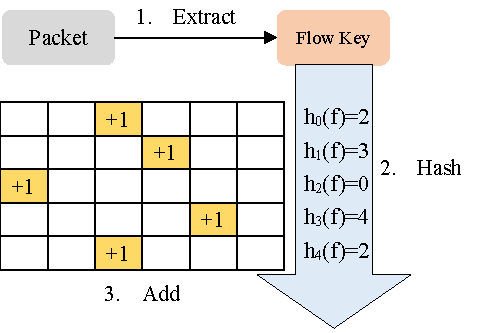
\includegraphics[width=0.7\linewidth]{fig/countmin2.pdf}
	\caption{Count-Min的更新过程}\label{fig:countmin}
\end{figure}

如图\ref{fig:countmin}所示,Count-Min sketch的存储形式是一个高度为$d$、长度为$w$的二维数组(这样的二维数组也称为\textit{bitmap})。数组中的每个位置称为一个“格子”(slot),格子中包含了一个从0开始的计数器。
数组中的每一行都拥有一个哈希函数,可以将任意流ID,如5元组,映射到$\{0,1,...,w-1\}$之间的某个整数。

当一个数据包到达时,Count-Min首先读取它的流ID,然后对于数组的每一行,使用它的哈希函数将ID映射为一个数,用这个数作为索引定位到相应的格子,将格子中的计数器增加对应的数据包大小。
由哈希函数的特性可知,同一条流的数据包将会一直映射到同样的$d$个格子。

要从Count-Min当中查询某个流的大小,先重复之前的步骤,利用哈希函数定位到具体的格子。因为Count-Min总共有$d$行,所以会找到$d$个格子。选择这些格子当中最小的计数器作为流的大小的估计。
由于哈希碰撞的存在,因此Count-Min的查询结果总是大于或等于实际的大小。

\subsection{CountSketch \cite{charikar2004finding}}\label{sec:countsketch}
CountSketch \cite{charikar2004finding}和Count-Min有一点相似,它同样拥有一个高度为$d$、长度为$w$的bitmap,以及$d$个将流ID映射成$\{0,1,...,w-1\}$中的整数的哈希函数。
除此之外,CountSketch还另有$d$个将流ID映射成$1$或$-1$的一系列哈希函数。

进行更新操作时,CountSketch首先使用第一套哈希函数来确定格子,再使用第二套哈希函数得到一个$1$或$-1$的系数。将数据包的大小乘上这个系数之后,再加到格子里的计数器上。
也就是说,Count-Min中的计数器只会增加,而CountSketch中的计数器有可能加也有可能减,取决于第二个哈希函数和流的ID。

在bitmap中查询流的大小的过程和Count-Min类似,但和Count-Min不同的是,CountSketch选择的不是$d$个计数值中的最小值,而是中位数。

\begin{figure}
   \centering
   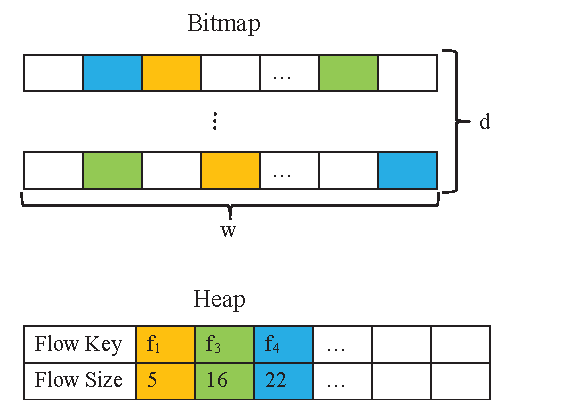
\includegraphics[width=0.7\linewidth]{fig/countsketch.pdf}
   \caption{CountSketch的结构}
   \label{fig:countsketch}
\end{figure}

此外,CountSketch还拥有找出top-$k$的流的能力。如图\ref{fig:countsketch}所示,为了记录top-$k$的流,CountSketch维护了一个容积为$k$的小根堆,其中存放了这些大流的ID以及它们的流量。

当数据包抵达时,CountSketch首先更新它的bitmap,然后再检查这个数据包所属的流是否已在堆中。
如果已在堆中,那么就将堆中对应的项目的流量值增加这个数据包的大小;
否则,CountSketch就会在bitmap中执行查询操作,获取当前流的流量估计值。
如果估计值比小根堆中最小的值要大的话,就将这个最小值移出堆,并将当前流的ID和流量估计值加入堆中。或者如果堆还没有满,也会当前流的信息放入堆中。

由于CountSketch的更新过程涉及堆的操作,因而它的计算负载也受堆操作的影响。如果使用简单的小根堆实现,那么更新堆中项目的时间复杂度是$O(\log{k})$, 在堆中查找某条流的时间复杂度是$O(k)$。
对每个数据包,CountSketch都要在堆中进行查找操作,这一过程大幅增大了CountSketch的计算负载。



\subsection{Filtered Space-Saving \cite{homem2010finding}}\label{sec:FSS}
在严格意义上,Filtered Space-Saving (FSS) \cite{homem2010finding}并非sketch,而应看做是一种基于“Counter”的算法,不过这个区别对于实际应用来说是可以忽略的。

FSS由一个只有1行的bitmap和一个容量为$k$的哈希表组成,其中bitmap用于粗略估算流的大小,哈希表则用来精确统计一部分的流的大小。
bitmap中的每个格子包括“计数器”和“指示器”两个字段。计数器用来记录流量统计,指示器则记录了通过哈希函数映射到这个格子中的流当中,有多少条也在哈希表当中。

每当新的数据包抵达,FSS首先用哈希函数将流的ID映射到bitmap中的一个格子,并检查这个格子中的指示器。
如果指示器的数字不为0,FSS会在哈希表中搜索该流ID。若流ID存在于哈希表中,那么哈希表中对应的计数器就增加数据包的大小。
如果指示器是0,或者ID不存在在哈希表中,那么就将bitmap中对应的格子里的计数器增加数据包的大小。
在此之后,若格子中的计数器大于哈希表中的最小值,就将该流的ID和计数器的数字插入哈希表中,并将格子中的指示器加1。
如果在插入时哈希表已满,那么哈希表中数值最小的一条流会被移除。在移除之后,FSS将会利用哈希函数为这条流找到它所对应的格子,将它原本在哈希表中的计数器数字复制到格子中的计数器中,并将格子里的指示器减1。

对于流ID存在于哈希表中的情况,FSS执行更新操作的时间复杂度是$O(1)$。其他情况下,FSS需要寻找哈希表中的最小项,因此时间复杂度是$O(k)$。


\subsection{SketchVisor \cite{huang2017sketchvisor}}\label{subsec:sketchvisor}

SketchVisor \cite{huang2017sketchvisor}论文为其中的“Fast Path”设计了一个可以实现top-$k$流统计的算法。此算法维护一个有$k$行的表,表中的每一行包含一个流的ID和3个统计字段。
每到达一个数据包,如果该数据包的流存在于表中,或者表尚未存满,则只是简单的在表中插入或增加对应的表项。否则,整张表内的所有数据都要更新,这种操作被称为“kick-out”。
\cite{huang2017sketchvisor}中的测试结果显示,一个kick-out操作需要12332个CPU时钟周期,普通的更新则只需要47个时钟周期。

根据这一测试结果,我们估算了不同的kick-out比率下处理每个数据包消耗的平均时钟周期数。
如表\ref{tbl:sketchvisor}所示,SketchVisor的计算负载只在kick-out比率不超过1\%时才能够接受。也就是说,SketchVisor的表中所存储的流的流量之和要超过全部流量的99\%。
在实际网络中,由于流是在变化的,用一张表追踪99\%的流量明显不切实际。更何况要囊括更多的流,$k$也要随之增大,导致占用的内存空间也会增大。

\begin{table}[h]
	\centering
	\caption{SketchVisor的计算负载随kick-out频率的变化}\label{tbl:sketchvisor}
	\begin{tabular}{c|c}
		\hline
		Kick-out 频率 & CPU周期/数据包 \\
		\hline
		0.1\% & 59 \\
		\hline
		0.5\% & 108 \\
		\hline
		1\% & 170 \\
		\hline
		2\% & 293 \\
		\hline
		5\% & 661 \\
		\hline
	\end{tabular}
\end{table}

\subsection{已有sketch所存在的问题}


在介绍了Count-Min等4种sketch之后,我们对这些sketch的优势和不足进行分析。

Count-Min的主要优势在于它的计算负载极低,并且估计误差较低。但是Count-Min并不记录任何流本身的信息,因而无法筛选出大流。一些研究对Count-Min进行了拓展,使其能够反查大流的信息。
如Deltoid \cite{cormode2005s}使用了额外的计数器来编码流的ID;
Reversible Sketch \cite{schweller2007reversible}将流ID拆分成多个部分并分别进行哈希;
FlowRadar \cite{li2016flowradar}使用连续的异或运算来编码和恢复流的ID。
然而,根据SketchVisor \cite{huang2017sketchvisor}中的测试结果,这些改进算法的计算负载都比较高。

SketchVisor有着较高的流量统计精度,然而它的计算负载取决于kick-out出现的频率。
随着kick-out比率的增加,SketchVisor的计算负载迅速增加并且变得无法负担。因而SketchVisor无法胜任大多数的应用情景。

CountSketch和FSS都使用了辅助数据结构,最坏情形下的更新操作的时间复杂度是$O(k)$。
第\ref{sec:simulation}节当中提供了一种用空间换时间的实现,使得最坏情形的时间复杂度降为$O(\log{k})$。
这个结果看起来似乎是可接受的,然而第\ref{sec:simulation}节中的模拟结果显示,这两种$O(\log{k})$的sketch的计算负载对于承载大量数据的交换机而言还是太大了。

我们用一个例子来帮助理解交换机的CPU资源与sketch的计算负载之间的关系。
假设一个交换机拥有24个端口,每个端口的速度都是10Gbps。所有端口的平均负载率记为$\beta$,这里假设$\beta$是0.2。数据包的平均大小是1KB。
可得交换机每秒要处理的数据包数约是:
\begin{equation}%\notag
    N = (10\times 10^9\cdot 24 \cdot \beta)/(0.5\times 10^3 \times 8) = 1.2\times 10^7
\end{equation}

在这样的假设下,如果sketch要处理经过交换机的所有数据包,那么sketch的吞吐量至少要能达到每秒1200万个数据包。
第\ref{sec:proto}节中我们对CountSketch和FSS的速度进行了测试,结果显示CountSketch和FSS处理一个数据包所需的CPU时钟周期数分别是约170和110。
假设这个交换机的CPU主频是1.5GHz,有2个物理核心(在市面上的交换机当中已经属于高端配置,相当于Juniper QFX5100系列\cite{juniper2018qfx5100}),CountSketch和FSS分别占用了68\%和44\%的CPU时间。
事实上,交换机的CPU还要承担其他的一些工作,比如流表操作、管理界面等。这些工作的优先级很有可能比流量测量更高,使得能够分配给sketch的计算资源更少。
而且,在实际应用中,$\beta$的数值很有可能比0.2要大,这也要求了sketch的计算负载必须更低。



\section{流量测量的分布式部署}

如第\ref{sec:measurement}节所述,现有的基于流表的统计方式中,每个交换机都会统计经过它的所有数据包。
这种方法的可行性源于流表在数据包处理中不可或缺的地位:所有数据包到达时都要匹配流表,在匹配到的同时顺便更新统计数据。
也就是说,即使交换机不再进行流量统计,流表匹配仍旧是必须进行的,因而基于流表的流量统计带来的计算负载实际上微乎其微。

和流表相比,sketch面临的性能瓶颈要严重的多。
在第\ref{sec:observation}节当中我们假设,一个交换机需要每秒用一个双核1.5GHz的CPU处理1200万个数据包,即达到12Mpps(Packet per Second)的吞吐量。
但是对于交换机而言,每秒12M个数据包只能算是极低的工作负载。
例如Juniper QFX5100系列交换机配备了和\ref{sec:observation}节的例子中相同的双核1.5GHz的CPU,
然而根据其规格手册,该系列中所有型号的吞吐率都超过了10亿pps\cite{juniper2018qfx5100},相当于上述假设的近100倍。
部分型号更是达到了14.4亿pps的吞吐量。
通过简单的计算便可得出,要想让sketch能够在这颗CPU上达到10亿pps的吞吐量,处理每个数据包不能花费超过3个时钟周期。
Sketch是部署在SRAM上的,以Intel Haswell处理器为例,在L1缓存的SRAM上读取数据最快也需要4个时钟周期\cite{hammarlund20134th},因而在3个时钟周期内处理一个数据包显然是不可能的。

另一种思路则是减少sketch要处理的数据包数,也就是分布式部署。
如果sketch不加区分地处理所有经过交换机的数据包,势必会带来巨大的冗余,造成计算资源的浪费。
在很多分层拓扑结构(如Fat-tree \cite{al2008scalable}和Spine-Leaf \cite{alizadeh2013data})中,所有流都按照接入层——汇聚层——接入层,至少经过3个交换机进行路由。
如果能将流量测量均匀分配到每个交换机中,减少冗余的测量,就能够降低单个交换机上的计算负载。
此外,当网络中的流量实在太大,sketch无论如何都无法处理的时候,必须对sketch消耗的资源量进行限制,优先保证交换机的基本功能。
因而我们还需要进行取舍,放弃对一部分流的测量以维持交换机的正常运行。
如何在交换机之间分配流量测量、如何对流进行取舍,这些问题构成了流量测量的分布式部署问题。

流量测量的分布式部署问题与一个现有问题非常相似,即流统计收集问题(Flow Statistics Colletion, FSC)。
FSC问题的背景是:所有交换机都使用流表统计了经过自己的所有流的流量信息,控制器要有选择地收集这些信息,以免造成过大的控制链路负载和信息延迟。
例如,在一个中等规模的数据中心网络中\cite{kannan2013compact},一个连接着40个服务器的交换机每分钟经过的流可能会有7.5到10万条。
如果要将所有统计信息都上报的话,首先根据DevoFlow \cite{curtis2011devoflow}中的研究,收集统计信息会对交换机的性能产生较大影响。
其次,按照第\ref{subsec:memory}节中的分析,即使上报的报文中只包含五元组的流ID和流量大小,其大小也有约1.5到2.2MB。
如果加入流的起止时间、数据包数,则报文大小会达到3到4MB。假设控制链路的带宽是100Mbps,传输报文需要约0.5秒的时间。
在控制器方面,若网络中有50台交换机,每进行一次统计信息的收集就会产生约200MB的数据,控制器需要对这些数据全部进行处理。
显然,由于一条流会经过多个交换机,这些数据当中包含了大量的冗余信息。
如果能够在上报前就剔除掉这些冗余的信息,就能够大幅降低交换机、控制器以及控制链路的负载。

FSC问题与流量测量部署问题可以看成是一个问题的正反两面:
FSC问题的目标是,交换机上无差别测量全部的流,但是有选择地上报流量信息;
而流量测量部署问题的目标则是从一开始交换机就有选择地进行测量。
因而,我们可以借鉴FSC问题的解决方案来解决流量测量部署问题。

FSC问题主要有三种解决方案:\emph{per-flow} \cite{van2014opennetmon}、\emph{per-switch} \cite{su2014flowcover}\cite{su2015cemon}和基于掩码(wildcard)的方案\cite{xu2017miniming}。
per-flow方案中控制器每次只查询一条流,对控制链路的负载较高,而且在流量测量部署问题当中,我们没办法预先知道网络中会有那些流,因而不合适;
per-switch方案则是选择若干个交换机,收集它们的全部统计数据。对应在流量测量部署问题中就是要这些交换机测量所有经过的数据包,这和我们问题的初衷相违背,因而也不合适。
掩码方案会为每个交换机下发一系列规则,当交换机收到控制器的流统计收集指令时,只上报符合这些规则的流的信息。
对于流量测量部署问题,我们也可以预先为交换机下发规则,交换机只测量符合规则的流的流量。因此,掩码方案是最适合流量测量部署问题的。


% 第\ref{sec:coop}节提出了一个协作式的简单的部署策略,确保每条流只会被测量一次,从而将计算负载均摊到入口和出口交换机。然而协作式部署最多只能降低50\%的计算负载,仍然不足以解决问题。

\section{本章小结}


本章首先分析了4种已有sketch的不足,主要是大流识别和计算负载的问题。
表\ref{tbl:sketchcompare}总结了Count-Min, CountSketch和FSS在不同方面的性能,以及我们设计的sketch应当具有的性能。
随后本章讨论了流量测量的分布式部署,通过和FSC问题类比,我们确定采取使用掩码的方案。


\begin{table*}[ht]
	\centering
	\caption{不同sketch之间的对比}\label{tbl:sketchcompare}
	\begin{tabular}{c|c|c|c|c}
		\hline
		sketch名称 & 计算负载 &估计误差&大流监测率& 能否识别大流 \\
		\hline
		Count-Min\cite{cormode2004improved} & 低 &低& 无 &否\\
		\hline
		CountSketch\cite{charikar2004finding} & 高 &高 &低&是\\
		\hline
		Filtered Space-Saving\cite{homem2010finding}  & 一般 & 一般&高& 是\\
		\hline
		\textbf{本文设计的sketch} & 低 &低 &高&是\\
		\hline		
	\end{tabular}
\end{table*}
%\chapter{CountMax:数据平面的流量测量工具}
\chapter{SDN中流量测量sketch的研究现状}

本章将介绍4种典型的用于流量测量的sketch,并分析它们为何无法适用于SDN。

\section{Count-Min\cite{cormode2004improved}}

\begin{figure}[h]
	\centering
	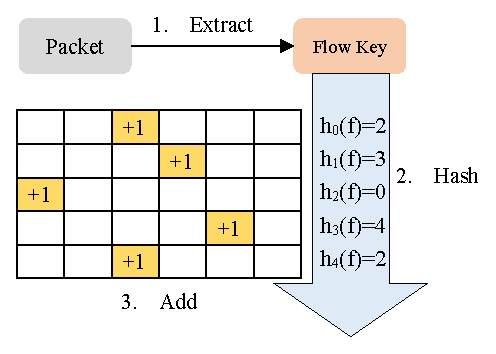
\includegraphics[width=0.8\linewidth]{fig/countmin2.eps}
	\caption{Count-Min的更新过程}\label{fig:countmin}
\end{figure}

如图\ref{fig:countmin}所示,Count-Min sketch的存储形式是一个高度为$d$、长度为$w$的二维数组(也称为\textit{bitmap})。数组中的每个位置称为一个“格子”(slot),格子中包含了一个从0开始的计数器。
数组中的每一行都拥有一个哈希函数,可以将任意流ID,如5元组,映射到$\{0,1,...,w-1\}$之间的某个数。

当一个数据包到达时,Count-Min首先读取它的流ID,然后对于数组的每一行,使用它的哈希函数将ID映射为一个数,用这个数作为索引定位到相应的格子,将格子中的计数器增加。
在统计数据包数的情况下,将计数器加一;在统计数据流量的情况下则将计数器增加相当于数据包字节数的大小。


\section{算法设计}
首先我们确定CountMax算法设计的目标,然后再来介绍算法的具体设计。
CountMax的算法设计包含两部分,其一为统计信息的记录和更新,其二为统计信息的查询。

\subsection{设计目标}
根据第\ref{chap:sketch}章中对已有的sketch方案的分析,为了解决已有sketch的不足,CountMax的设计目标有以下几点:
\begin{enumerate}
	\item 大流识别。在实际应用中我们很难获得关于大流的先验知识,因此CountMax必须负责将大流的ID从成千上万的流当中识别出来。
	\item 更低的计算负载。CountMax应当占用尽可能少的CPU资源,一方面可以应对更重的网络负载,另一方面也为交换机上的其它应用留出了空间。
	\item 较低的测量误差。CountMax对大流流量的估算误差应当可控,且处于可接受的较低范围内。
	\item 追踪更多的大流。在消耗同样的存储空间的前提下,被CountMax所追踪的大流越多,就可以提供越多的有用信息,提升重路由等应用的质量。
\end{enumerate}

\subsection{设计简述}
为了尽量降低计算负载,CountMax摒弃了提高复杂度的辅助数据结构。我们选择仿照Count-Min的设计,只使用bitmap存储数据。
同时,为了识别大流,CountMax在bitmap的每一个格子中都增加了一个存放流ID的字段。
当发生哈希冲突时,Count-Min不对流做区分,全部累加到计数器当中。这样的做法导致了Count-Min无法记录大流的ID。
因此,在CountMax的设计中,在多条流发生哈希冲突时,会根据当前流的ID和bitmap中现有的流ID的关系来选择不同的操作。
可简要描述为:若二者相同,则计数器增加;若二者不同,则计数器减去相应的大小。若减去后的结果为负数,对应格子中的流ID字段也会更改为当前流的ID。
由于网络中的大流的大小往往是小流的上千倍,当一条大流和多个小流碰撞时,这样的算法可以在绝大多数情况下保证最终记录下来的流ID是大流的ID。
而对于大流之间的哈希碰撞,则可以通过增加bitmap行数的方式降低其概率。

\subsection{统计信息记录}
为了记录统计信息,我们维护一个有$d$行、$w$列的bitmap。
Bitmap中的每个格子包含两个字段:$Key$和$Counter$。参数$d$和$w$的意义将在后文讨论。
和bitmap一起的还有$d$个不同的哈希函数$\{h_{1},...,h_{d}\}$。
每个哈希函数$h_j$都能将任意流的ID(如五元组)单向映射为一个介于$0$和$w-1$之间的整数:
\begin{equation}
\notag h_j: \{...\} \to \{0, ..., w-1\}
\end{equation}

\begin{algorithm}[htb]
    \small
    \SetAlgoLined
    \KwData{$f_i$:流的ID; $c_i$:数据包的大小}
  
    \For{$j$从0到$d-1$}{
        $u_j = h_{j}(f_i)$\;
        $f' = Key_{j}[u_j]$\;
        \eIf{$f_i == f'$}{
            $Counter_{j}[u_j] = Counter_{j}[u_j]+c_i$\;
        }{
            \If{$Counter_{j}[u_j] > c_i$}{
                $Counter_{j}[u_j] = Counter_{j}[u_j]-c_i$\;
            }{
                $Counter_{j}[u_j] = c_i-Counter_{j}[u_j]$\;
                $Key_{j}[u_j] = f$\;
            }
        }
    }
    \caption{CountMax对每个数据包的处理过程}
    \label{alg:count_max}
\end{algorithm}
当交换机接收到第$i$号数据包时,首先从数据包中解析出流的ID,记为$f_i$。对于bitmap中的第$j$行,先计算$f_i$的哈希值$u_{j}=h_{j}(f_i)$作为索引。
如果$Key_{j}[u_{j}]$与$f_i$相同,那么对应的$Counter_{j}[u_{j}]$就会加上数据包的大小,记做$c_i$。否则比较$Counter_{j}[u_{j}]$和$c_i$之间的大小。
如果$Counter_{j}[u_{j}]$\textbf{大于}$c_i$,那么$Counter_{j}[u_{j}]$就减去$c_i$。写成表达式即为$Counter_{j}[u_{j}] = Counter_{j}[u_{j}] - c_i$。
如果$Counter_{j}[u_{j}]$\textbf{小于}$c_i$,则令$Counter_{j}[u_{j}]=c_i - Counter_{j}[u_{j}]$,并且将$Key_{j}[u_{j}]$替换为$f_i$。

对bitmap中的每一行迭代上述过程。算法\ref{alg:count_max}详细描述了这一算法。

\subsection{流量信息查询}
%\input{query.tex}
要查询流$f_i$的统计信息,首先从每一行中分别查询。对于sketch中的第$j$行,采用如下的方法获取$f_i$在当前行内的估计$\hat{a}_{i_{j}}$:
\begin{equation}
\hat{a}_{i_{j}}=\left\{
\begin{aligned}
Counter_{j}[h_j(f_i)]&\text{, 若 $f_i=Key_{j}[h_j(f_i)]$}\\
0&\text{, 若 $f_i \ne Key_{j}[h_j(f_i)]$}
\end{aligned}
\right.
\end{equation}

要推断流的流量大小,我们用上述方法查询每一行,从得到的结果中选取最大值作为估计值。
\begin{equation}
\label{eq:query}
\hat{a}_{i}=\max{\{\hat{a}_{i_{j}} , \forall j\}}
\end{equation}

\section{算法分析}\label{sec:analysis}
\label{subsec:analysis}
%\input{analysis.tex}

CountMax具有找出大流的能力。在分析CountMax的具体性能之前,首先对“大流”进行定义。
在网络中,随着流量分布的变化,字面意义上的top-$k$,即网络中流量最大的$k$条流的特征很难量化。因此,我们采用“heavy hitter”作为大流的定义。

给定网络中的所有流的集合,其中总共有$n$条流,所有流的流量之和是$F$。给定一个参数$\delta$ ($0<\delta \le 1$),则每一条流量大于或等于$\delta\cdot F$的流就称为这个集合中的$\delta$-``heavy hitter"。

\subsection{近似性能分析}
本小节将证明,在一定概率内,CountMax可以对heavy hitter的估计值有着可控的近似比。

\begin{theorem}
	\label{tm:query}
    对每条$\delta$-heavy hitter流$f_i$,令$\hat{a}_i$和$a_i$分别表示$f_i$的估算流量和实际流量。
    令$\tilde{d}$表示bitmap中记录有$f_i$的行的数目(即满足$Key[h(f_i)] = f_i$的行数),$e$代表自然对数的底,如下不等式始终满足:
	\begin{equation}
	\label{eq:hhacc}
	Pr[1-\frac{e}{w\cdot \delta}\le \frac{\hat{a}_i}{a_i} \le 1] \ge 1-e^{-\tilde{d}}
	\end{equation}
\end{theorem}

\begin{proof}
首先,由CountMax的性质易知,$\hat{a}_i$始终不大于$a_i$,即:
\begin{equation}
    \hat{a}_i/{a_i} \le 1
\end{equation}

接下来引入变量$I_{i,k,j}$来指示$f_i$和$f_k$两条流是否在第$j$行发生哈希冲突。即:
\begin{equation}
    I_{i,k,j}=\left\{
    \begin{aligned}
    1&\text{, if ($f_i \ne f_k $ ) $\land $ ($h_j(f_i)=h_j(f_k)$)}\\
    0&\text{, otherwise}
    \end{aligned}
    \right.
\end{equation}
由于哈希函数在理论上是独立的,因此对$f_i$和$f_k$的哈希计算可视为两个独立实验。又因为对不同的输入,理想的哈希函数将其散列到每个格子的概率是均等的,因此有:
\begin{equation}
    E(I_{i,k,j})=Pr[h_j(f_i)=h_j(f_k)] = \frac{1}{w}
\end{equation}

接下来定义变量$X_{i,j}$,令其表示在第$j$行中和$f_i$产生了哈希冲突的所有流的流量之和。即:
\begin{equation}\label{eq:xij}
    X_{i,j}=\sum\nolimits_{k=1}^{n}I_{i,k,j}\cdot a_k
\end{equation}

由于当$Key[h_j(f_i)]\ne f_i$时,查询的结果是0,因此必须找到$Key[h_j(f_i)] = f_i$的充分条件。
对于第$j$行,如果 $a_i > X_{i,j}$,也就是$a_i$大于这个格子所处理的总流量的一半,根据鸽巢原理,无论数据包的到达顺序如何,$Key[h_j(f_i)]$ 都必然是 $f_i$,并且$Counter[h_j(i)]\ge a_i-X_{i,j}$。
也就是说,对于$f_i$而言,$\tilde{d}$大于等于满足$a_i > X_{i,j}$的行的数量。
另外,如果$a_i \le X_{i,j}$,因为$Counter[h_j(i)]$永远不会为负,因此$Counter[h_j(i)]\ge a_i-X_{i,j}$依旧成立。

\begin{equation}\label{eq:ai_xij}
    Counter[h_j(i)]\ge a_i-X_{i,j}
\end{equation}

根据等式\eqref{eq:xij}可得:
\begin{equation}\label{eq:ex}\notag
E(X_{i,j})=E(\sum_{k=1}^{n}I_{i,k,j}\cdot a_k)\le\sum_{k=1}^{n} a_k\cdot E(I_{i,k,j})\le \frac{1}{w}\sum_{k=1}^{n}a_k.
\end{equation}


再根据$\delta$的定义,若$f_i$是$\delta$-heavy hitter,则网络中的总流量不超过$\frac{a_i}{\delta}$。因此:
\begin{equation}\label{eq:ex-delta}
E(X_{i,j})\le \frac{1}{w}\sum_{k=1}^{n}a_k\le \frac{1}{w}\cdot \frac{a_i}{\delta}
\end{equation}

综合以上结论,可以进行如下的推导。为方便起见,“$\forall j$”在这里代表“ $\forall j\in \{j|Key[h_j(f_i)] = f_i\}$”。
\begin{align}\notag
&Pr[\hat{a}_i< a_i-\frac{e}{w}\cdot\frac{a_i}{\delta}]\\\notag
&=Pr[\forall j, Counter[h_j(f_i)]<a_i-\frac{e}{w}\cdot\frac{a_i}{\delta} ]\\\notag
&\le Pr[\forall j, a_i-X_{i,j} <a_i-\frac{e}{w}\cdot\frac{a_i}{\delta} ] \text{ (根据不等式\eqref{eq:ai_xij})}\\\notag
&=Pr[\forall j, X_{i,j} > \frac{e}{w}\cdot\frac{a_i}{\delta} ]\\\notag
&\le Pr[\forall j, X_{i,j}>e\cdot E(X_{i,j})]\text{\ \ (根据马尔可夫不等式)}\\\notag
&<e^{-\tilde{d}}
\end{align}
	
将该不等式左侧的条件取反,可得结论:
\begin{equation}
Pr[\frac{\hat{a}_i}{a_i} \ge 1-\frac{e}{w\cdot \delta}]\ge 1-e^{-\tilde{d}}
\end{equation}

定理\ref{tm:query}得证。
\end{proof}


接下来分析$\tilde{d}$的数学期望。

\begin{theorem}\label{tm:acc}
对任何$\delta$-heavy hitter,$E[\tilde{d}]\ge d\cdot(1-1/(w\cdot\delta))$。
\end{theorem}

\begin{proof}
对于$\delta$-heavy hitter流 $f_i$以及bitmap中的第$j$行,根据上一节的推断,如果$a_i > X_{i,j}$那么$Key[h(f_i)] $ 一定为 $f_i$。

根据马卡洛夫不等式和不等式\eqref{eq:ex-delta},可得:
\begin{align}\notag
	Pr[X_{i,j}>a_i] &\le \frac{E[X_{i,j}]}{a_i}\\\notag
	&\le \frac{1}{w}\cdot\frac{a_i}{\delta}\cdot\frac{1}{a_i}\\
	&\le \frac{1}{w\cdot\delta}
\end{align}
因此 $Pr[Key[h_j(f_i)]=f_i]\ge 1- Pr[X_{i,j}>a_i] \ge 1-\frac{1}{w\cdot\delta}$。
    
由于bitmap中的每一行是独立的,因此$E[\tilde{d}]\ge d\cdot(1-1/(w\cdot\delta))$。
\end{proof}

\subsection{时间复杂度分析}
\begin{theorem}\label{tm:time}
CountMax对一个数据包进行处理的过程的时间复杂度是$O(d)$。
\end{theorem}

\begin{proof}
由于每一行的操作是固定的一次哈希、一次比较、一次加法,因而每行的时间复杂度是$O(1)$。
CountMax总共有$d$行,所以时间复杂度是$O(d)$。
\end{proof}




\section{CountMax在SDN中的应用}
本节介绍使用CountMax在SDN中进行重路由的应用,还提出了一种协作式的部署方式。
\subsection{借助CountMax进行重路由}\label{sec:flowrerouting}
流的重路由对于许多实际应用都是必要且十分重要的,如链路负载均衡以及链路中断时的重新寻路\cite{xu2017incremental}
。对于这些应用,网络中的大流的流量统计信息更加重要\cite{xu2017scalable}。

通过周期性地收集交换机的统计数据,控制器可以监控链路的流量负载。当控制器发现某条链路负载过重时,就需要对流进行重路由。
如果在交换机上安装了CountMax,控制器就可以收集CountMax中的信息,从而找出大流的集合,记为 $\Gamma^e$。
由于大流的流量占据了了网络整体流量中的大部分,因此通过采用各种算法对这些大流进行重路由,就可以快速有效地优化链路负载。
例如,我们可以利用一个简单的贪心法来重路由这些大流。首先将大流按照流量降序排列,然后按照顺序,控制器对每条流寻找一个占用率最低的路径作为新的路由。
在为所有大流都找好了新路径之后,将这些路径下发到交换机中\cite{jin2014dynamic} \cite{xu2017joint}。

这一过程中只对大流进行了重路由,而大流的数量和网络中流的总数相比非常少,因此重路由所需的时间也大幅减少。
由于CountMax的存储占用很小,因此收集CountMax的信息也不会为控制器带来明显的负载。


% \section{近似性能和计算负载的初步模拟}
% 小节\ref{sec:analysis}中的分析当中多次使用了不等式缩放、马尔可夫不等式,因此最终得到的结论颇为宽松。
% 为了更清楚的了解CountMax的实际性能,我们用C语言实现了CountMax并进行了一系列模拟。关于模拟环境的详细介绍请参见第XXXX章。
\begin{figure}[h]
	\centering
	\begin{minipage}[t]{0.48\linewidth}		
		%\begin{figure}[!t]
		\centering
		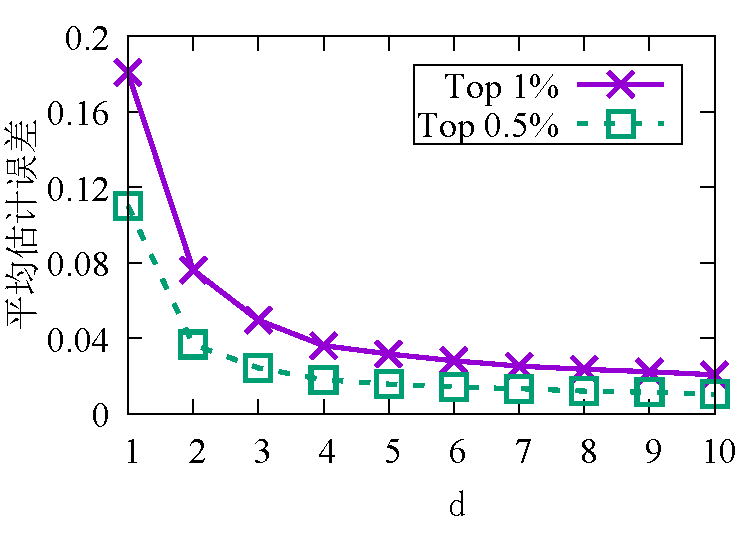
\includegraphics[width=\linewidth]{fig/cm_d_err.pdf}
		\caption{\textnormal{CountMax近似误差与$d$的关系}}
		\label{fig:cm,d,acc}
		%\end{figure}
	\end{minipage}\vspace{-0.6em}
\hspace{0.4em}
	\begin{minipage}[t]{0.48\linewidth}
        \centering
		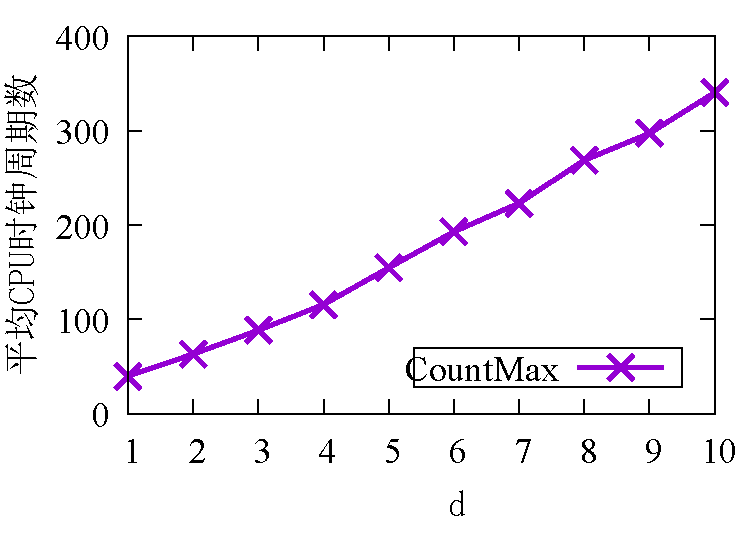
\includegraphics[width=\linewidth]{fig/cm_d_cpu.pdf}
		\caption{\textnormal{CountMax处理一个数据包的平均CPU周期数}}
		\label{fig:cm,d,cpu}
	\end{minipage}\vspace{-0.6em}
\hspace{0.1em}
\end{figure}

\subsection{CountMax的协作式部署}\label{sec:coop}
要进一步降低CountMax在交换机上的计算负载,主要有两种方法。
根据定理\ref{tm:time},CountMax处理单个数据包的时间复杂度是$O(d)$,因此第一种方法就是通过减少$d$的值来降低计算负载。

图\ref{fig:cm,d,acc}描述了CountMax在不同的行数下,对网络中前1\%或0.5\%的流的流量估计的误差。
关于测试环境的具体介绍请参见第\ref{sec:simulation}节。图\ref{fig:cm,d,acc}中的测试对应的是其中Spine-Leaf拓扑、20万条流、$k=2000$、非协作式的情况。
由图中我们可以看到,随着$d$的增长,估计误差一开始迅速降低,但随后降低的速度大幅放缓。$d=3$时的误差和$d=10$时的误差差别很小。
当$d=2$时,误差已经控制在10\%以内。

图\ref{fig:cm,d,cpu}描述了CountMax处理数据包所需的CPU时钟周期随$d$的变化而变化的情况。
图中的结果显示,CountMax的处理一个包的计算负载和$d$大致呈线性增长,同时印证了定理\ref{tm:time}。

\begin{figure}[h]
   \centering
   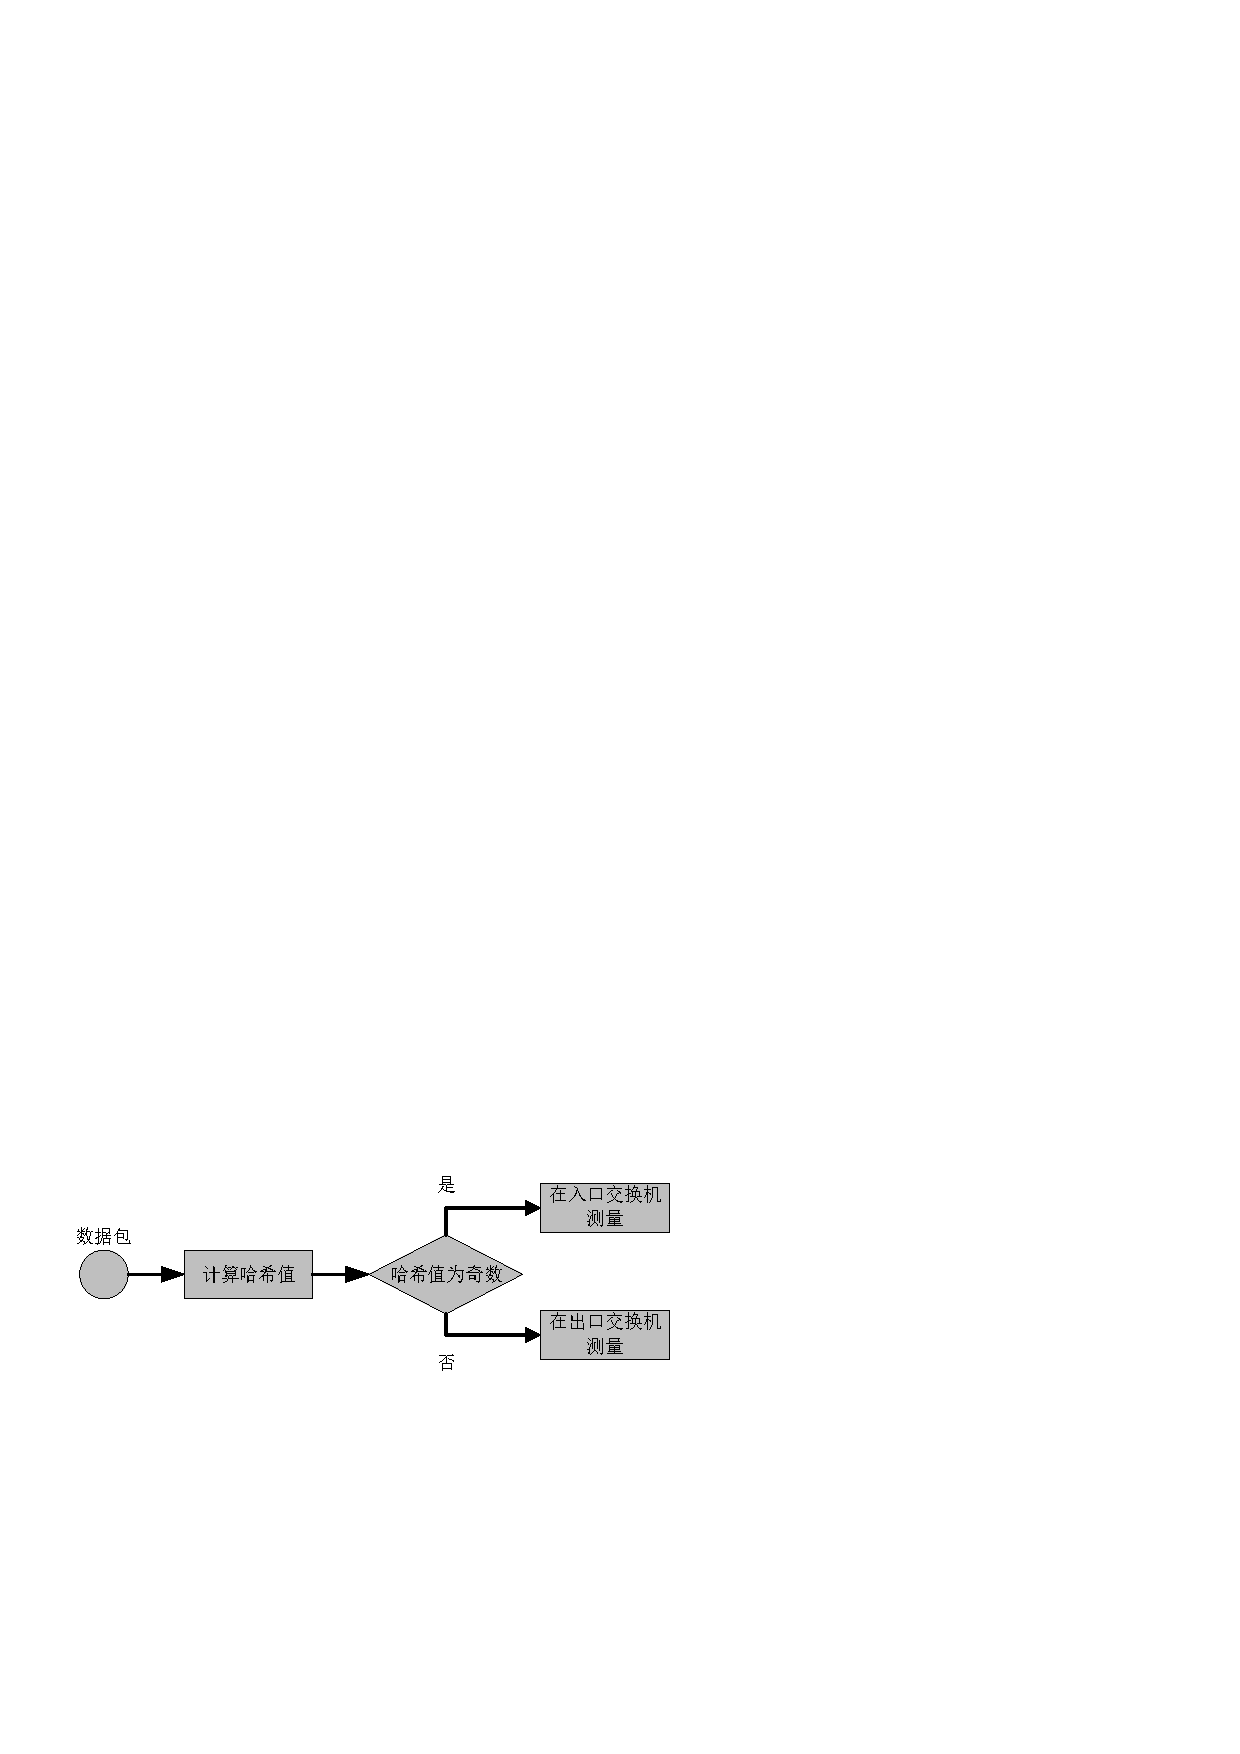
\includegraphics[width=0.7\linewidth]{fig/filter_measure.pdf}
   \caption{协作式CountMax的示意图}
   \label{fig:filtermeasurement}
\end{figure}

另一种降低计算负载的方法是减少CountMax所需要处理的数据包的个数。要测量流的流量,最简单的方案就是在每一个交换机上都部署一个CountMax,并且处理经过交换机的所有数据包。
然而,网络中的很多流是要经过多个交换机的(由于CountMax的主要应用是流的重路由,所以实际上我们只关心那些要经过多个交换机的流),同一条流可能会被多个交换机统计,造成资源的浪费。

因此,本文提出了一种“协作”的方法,使用简单的方式保证一条流只会被一个交换机测量。协作式的流量测量的流程如图\ref{fig:filtermeasurement}所示。
每当一个数据包抵达交换机时,交换机首先用一个哈希函数对流的ID进行哈希。这个哈希函数是所有交换机所共享的。
如果哈希的结果是奇数,那么这条流应当被它的入口交换机,也就是路由上的第一个交换机进行测量。反之则被出口交换机所测量。
交换机可以通过这条流的入端口和出端口来判断自己是不是入口交换机或者出口交换机。
和第\ref{chap:gmsc}章中介绍的分布式部署方式不同,协作式CountMax是完全自组织的,无需控制平面的介入。

接下来分析协作式CountMax的估计误差。不失一般性,我们假设网络中只有两个交换机。网络中的所有流都是先经过交换机1,再经过交换机2的。
假设所有流的总流量是$F$,交换机1处理的流量占比是$\gamma_1 $,那么它处理的总流量就是$F_1 =\gamma_1\cdot F $。
相应的,交换机2处理的流量占比是$\gamma_2 $,总流量是$F_2 =\gamma_2\cdot F $。

首先关注交换机1。令$f$代表网络中所有的流当中的一条$\delta$-heavy hitter流,则$f$的流量大于$\delta \cdot F$。
如果$f$是被交换机1所处理的,那么对于被交换机所处理的流的集合而言,$f$是一个$\delta/\gamma_1$-heavy hitter。
根据定理\ref{tm:query}和定理\ref{tm:acc},有如下不等式成立:

\begin{equation}\label{eq:coop_acc}
\left\{
\begin{aligned}
&Pr[1-\frac{e\cdot \gamma_x}{w\cdot \delta}\le \frac{\hat{a}_i}{a_i} \le 1] \ge 1-e^{-\tilde{d}}\\
&E[\tilde{d}]\ge d\cdot(1-\frac{\gamma_x}{w\cdot\delta})
\end{aligned}
\right.
\end{equation}

其中$\gamma_x$ 根据这条流被哪个交换机所测量,而代表 $\gamma_1$ 或 $\gamma_2$。如果定义 $\gamma_m = \max \{\gamma_1, \gamma_2\}$,用$\gamma_m$替换$\gamma_x$,即可得到一个下界。
在最好的情况下,$\gamma_1=\gamma_2=1/2$。
在实际情况中,通过选择足够随机的哈希函数,$\gamma_1$ 和 $\gamma_2$通常都会比较接近。
参照等式\eqref{eq:coop_acc}, 协作式CountMax将$\frac{\hat{a}_i}{a_i}$ 和 $E[\tilde{d}]$ 这两个值的界缩紧为原本的 $\gamma_m $倍。

\chapter{仿真模拟与系统测试}
%\chapter{流量统计设施的部署}
在前几章,我们使用CountMax解决了数据平面上流量统计的获取问题,接下来我们从控制平面探讨流量统计该如何部署。

第\ref{sec:coop}节提出了一个协作式的简单的部署策略,将计算负载均摊给所有入口和出口交换机。
但是在现实网络中的情况更加复杂,简单的协作式很可能不能满足需求,因此我们寻求在控制平面进行更优化的部署。
\chapter{GMSC:流量测量的分布式部署算法}\label{chap:gmsc}
在第\ref{chap:countmax}章,我们使用CountMax解决了数据平面上流量统计的获取问题,并提出了一个无需控制平面干预的简易部署方式——协作式CountMax。

接下来我们从控制平面出发,更进一步地探讨流量测量的分布式部署。
本章首先对问题进行形式化建模和描述,随后提出了一种名为GMSC的解决算法,最后利用仿真模拟对其进行了测试。

\chapter{最大化流统计覆盖问题}
\chapter{GMSC:流统计覆盖的解决算法}\label{chap:gmsc}
在本章,我们提出一个简单但有效的算法解决MSC问题,称为GMSC。

\section{算法设计}\label{sec:gmsc}
如第\ref{sec:mscdef}节中定理\ref{thm:nphard}的证明,在只考虑交换机$v_i$的情况下,MSC问题退化为单背包问题。
我们可以对每个交换机分别求解单背包问题,获得每个交换机的最大容纳价值,记为$p(v_i)$。
接下来选择$p(v_i)$最大的那个交换机,将背包问题的解应用到此交换机上。
最后,由于这个交换机被分配了掩码,要相应的更新这些掩码在其余交换机上的价值。
重复这个过程,直到所有交换机都被分配过为止。

这是一个贪心(Greedy)算法,因而称其为GMSC。
\begin{algorithm}[htb]
    \small
    \SetAlgoLined
    \KwData{$V$:交换机的集合;$F$:覆盖的所有流的集合}
    $F=\Phi$\;
    \While{$|V|>0$}{
        \ForEach{$V$中的交换机$v$}{
            求解单背包问题,得到$v$的最大价值$p(v)$和对应的解$S(v)$。记$S(v)$中覆盖的流的集合为$F(v)$\;
        }
        找出$m$,使$p(v_m)$最大\;
        将$S(v_m)$中的掩码应用到$v_m$上\;
        将$F(v)$中覆盖的流加入$F$\;
        从$V$中移除$V_m$\;

        \ForEach{$V$中的交换机$v_i$}{
            \ForEach{$\Omega$中的掩码$r_j$}{
                更新$p(\Pi_i^j)$,去除$\Pi_i^j \cap F(v)$部分的价值\;
            }
        }
    }
    \caption{GMSC}
    \label{alg:count_max}
\end{algorithm}

\section{单背包问题的解法}
作为一个经典问题,单背包问题有多种不同的解法,其中最经典的是动态规划法 \cite{martello1999dynamic}和贪心法\cite{cmulec10}。
这两种解法在各类算法教科书中都能轻易找到,因此不再赘述。
设背包容量为$B$,可选择的物品数为$m$,则动态规划法的时间复杂度是$O(m\cdot B)$,近似比为1;
贪心法的时间复杂度是$O(m \log{m})$,近似比为1/2。

\section{GMSC的性能分析}
\subsection{近似性能}
\begin{theorem}\label{tm:gmscappr}
    GMSC的近似比为$\frac{\mu}{1+\mu}$,其中$\mu$为单背包问题解法的近似比。
\end{theorem}

\begin{proof}
令$Q_G$表示通过GMSC所覆盖的流,$G_l$表示GMSC在第$l$次迭代后所覆盖的流,则$Q_G = G_n$。
令$X_l$代表第$l$次迭代中所选择的掩码带来的价值增量,则$X_l =w(G_l \backslash \bigcup\nolimits^{l-1}_{i=1}G_i)$。

考虑GMSC已经完成$l-1$轮迭代的情况。在第$l$轮中,GMSC选择了交换机$v^l$和其上的流$X_l$。
作为对比,最优解法也一定会从$v^l$中选择一个掩码的集合,其中包含的流的集合记为$O_l$。
设最优解法最终覆盖的流的集合为$OPT$,则$OPT = \bigcup\nolimits_{l=1}^{n}O_l$。
如果在这一轮,我们选择$O_l$而不是$X_l$的话,则这一轮的价值增量为$w(O_l \backslash \bigcup\nolimits^{l-1}_{i=1}G_i)$,记为${X'}_l$。

设在已完成$l-1$轮的情况下,$v^l$上的背包问题的最优解是$Y_l$,则根据近似比的定义有$X_l \ge \mu Y_l$。
又因为$Y_l$是当前情况下的短视最优解,故$Y_l \ge {X'}_l$。
因而我们有:

\begin{align}
    X_l &\ge \mu Y_l \notag\\
        &\ge \mu {X'}_l \notag\\
        &= \mu \cdot w(O_l \backslash \bigcup\nolimits^{l-1}_{i=1}G_i) \notag\\
        &\ge \mu \cdot w(O_l \backslash Q_G) \notag
\end{align}

根据$Q_D$和$OPT$的定义,有:
\begin{align}
    w(Q_D)&=\sum\nolimits_{l=1}^{n} X_l \notag\\
        &\ge \sum\nolimits_{l=1}^{n} \mu \cdot w(O_l \backslash Q_D) \notag\\
        &=  \mu \cdot \sum\nolimits_{l=1}^{n} w(O_l \backslash Q_D) \notag\\
        &\ge \mu \cdot w ((\bigcup\nolimits_{l=1}^{n}O_l) \backslash Q_D) \notag\\
        &=  \mu \cdot w( OPT \backslash Q_D) \notag\\
        &\ge \mu \cdot [ w(OPT)-w(Q_D)] \notag
\end{align}

因而:
\begin{equation}\label{eq:gmscappr}
    w(Q_D) \ge \frac{\mu }{1+\mu} \cdot w(OPT)
\end{equation}
定理\ref{tm:gmscappr}得证。
\end{proof}

\section{时间复杂度}
若单背包问题的解法的时间复杂度为$O(\rho)$,更新一个掩码的价值的时间复杂度为$O(\tau)$,则GMSC的时间复杂度为$O(n^2\cdot m \cdot \tau + n^2 \cdot \rho)$。

假设一个掩码中最多有$h$个流,那么$\tau = h\cdot m$。因而:

\begin{theorem}\label{tm:gmsctime}
    GMSC的时间复杂度为$O(n^2\cdot m^2 \cdot h+ n^2 \cdot \rho)$。
\end{theorem}
\section{GMSC的仿真模拟测试}
本节使用仿真平台对GMSC的性能进行测试。具体而言,是测试GMSC能在多大程度上提升sketch测量的性能。

\subsection{测试设置}
本节中用到的测试指标为平均估计误差和最大交换机负载,
其中平均估计误差的定义与第\ref{subsec:metric}节相同。
最大交换机负载是统计每个交换机所处理的流量总和,取其最大值作为指标。
测试基准有两种,第一种是协作式CountMax,另一种是非协作式CountMax。
其中非协作式CountMax是在所有接入层交换机上都部署CountMax,每个CountMax只处理以本交换机作为出口交换机的数据包。
对于一条流被多次测量的情况,采取多个测量值的最大值作为结果。

测试拓扑采用的是与第\ref{sec:simulation}节相同的Fat-tree。
测试当中,用于计算的先验知识为所有流的准确信息和大小,掩码根据源地址与目的地址(O-D对)进行分割。
测试用的流的集合也与第\ref{sec:simulation}节相同,其中最大的一条流的大小约为9GB。
在GMSC中,每条流的价值和代价均为流的流量大小,每个交换机设置的负载上限约为10GB。

\subsection{测试结果}

\begin{figure}[ht]
	\centering
	\begin{minipage}[t]{0.48\linewidth}		
		%\begin{figure}[!t]
		\centering
		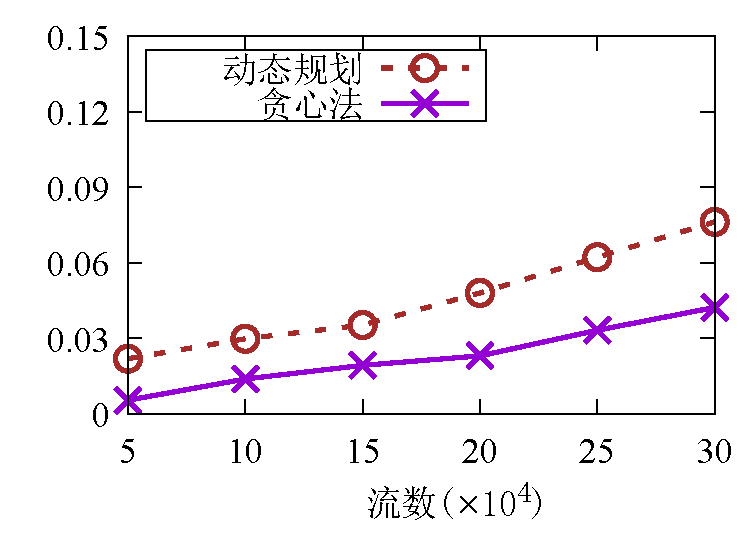
\includegraphics[width=\linewidth]{fig/msc_cmp_appr.pdf}
		\caption{\textnormal{平均估计误差与流数,$k=1000$。}}
		\label{fig:msc,appr}
		%\end{figure}
	\end{minipage}\vspace{-0.6em}\hspace{0.4em}
	\begin{minipage}[t]{0.48\linewidth}
		\centering
		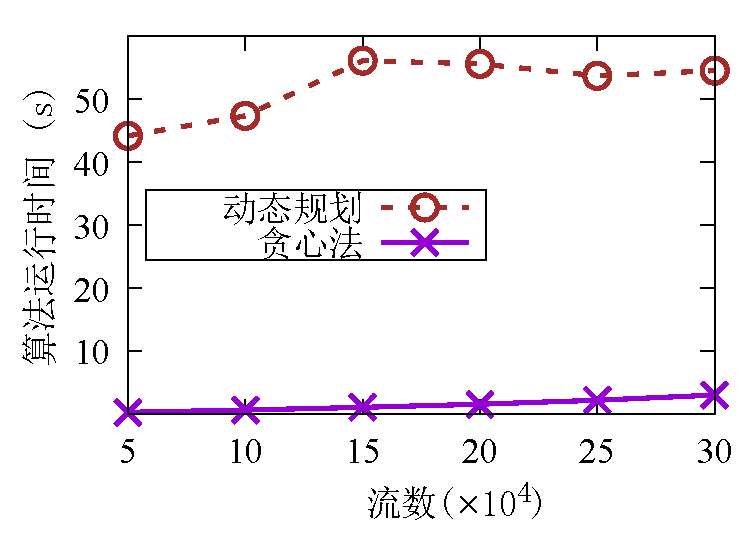
\includegraphics[width=\linewidth]{fig/msc_cmp_time.pdf}
		\caption{\textnormal{算法运行时间与流数,$k=1000$。}}
		\label{fig:msc,time}
	\end{minipage}\vspace{-0.6em}
\end{figure}

第一组测试是对比使用动态规划解背包问题的GMSC和使用贪心法解背包问题的GMSC的性能。
由于动态规划算法的时间复杂度和背包容量,即交换机负载上限呈线性关系,而测试中这一数字十分巨大,导致动态规划算法耗时极其漫长。
为了能够在合理的时间内获得结果,在这组测试中我们将流的价值和负载上限进行等比缩放(全部除以1000)后再进行动态规划。
图\ref{fig:msc,appr}中显示,由于缩放带来的误差,使用动态规划方法最终得到的估计误差反而超过了使用贪心法的误差。
图\ref{fig:msc,time}则表明,即使进行了1000倍的缩放,动态规划方法的运行时间仍是贪心法的10倍以上。
贪心法的运行时间随流数增加而增加的原因是,流数越多,每轮迭代后更新$p(\Pi_i^j)$所需的时间也会线性增加。

根据这一组实验的结果,我们决定接下来的测试中,GMSC一律使用贪心法解背包问题。

\begin{figure}[ht]
	\centering
	\begin{minipage}[t]{0.48\linewidth}		
		%\begin{figure}[!t]
		\centering
		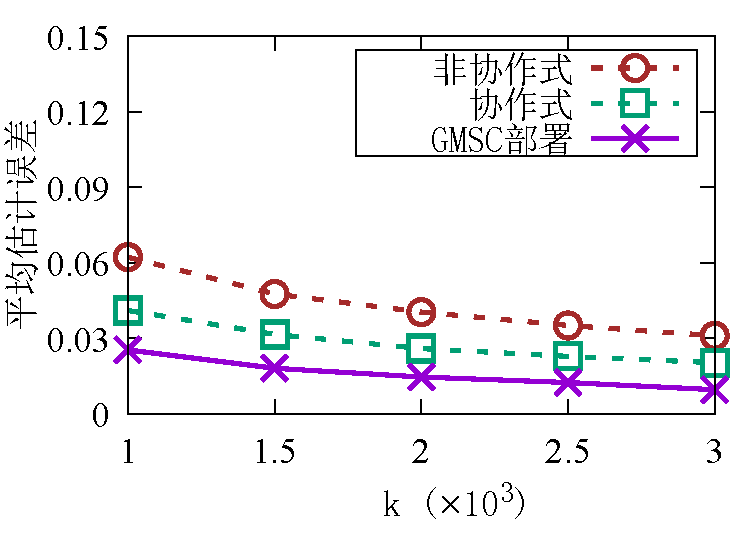
\includegraphics[width=\linewidth]{fig/msc_k_appr.pdf}
		\caption{\textnormal{平均估计误差与$k$,200000条流,$\alpha = 1\%$。}}
		\label{fig:msc,err,k}
		%\end{figure}
	\end{minipage}\vspace{-0.6em}\hspace{0.4em}
	\begin{minipage}[t]{0.48\linewidth}
		\centering
		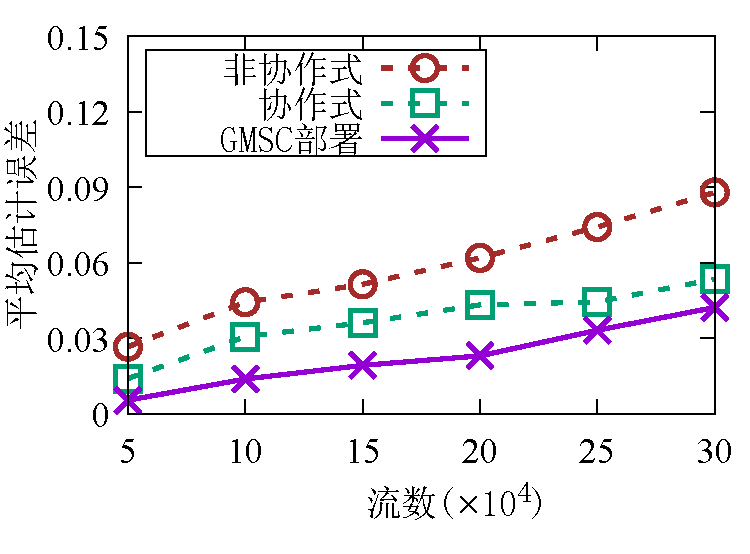
\includegraphics[width=\linewidth]{fig/msc_f_appr.pdf}
		\caption{\textnormal{平均估计误差与流数,$k=1000$,$\alpha = 1\%$。}}
		\label{fig:msc,err,flow}
	\end{minipage}\vspace{-0.6em}
\end{figure}

图\ref{fig:msc,err,k}和图\ref{fig:msc,err,flow}描述了使用GMSC部署的CountMax的估计误差与协作式和非协作式CountMax的对比。
在GMSC部署下,CountMax对网络中的大流的估计误差略有下降。和协作式CountMax相比约降低了20\%到30\%。
这主要是得益于GMSC部署将流的测量分散到各个交换机中,从而进一步减少了哈希冲突出现的概率。

\begin{figure}[ht]
	\centering
	\begin{minipage}[t]{0.48\linewidth}		
		%\begin{figure}[!t]
		\centering
		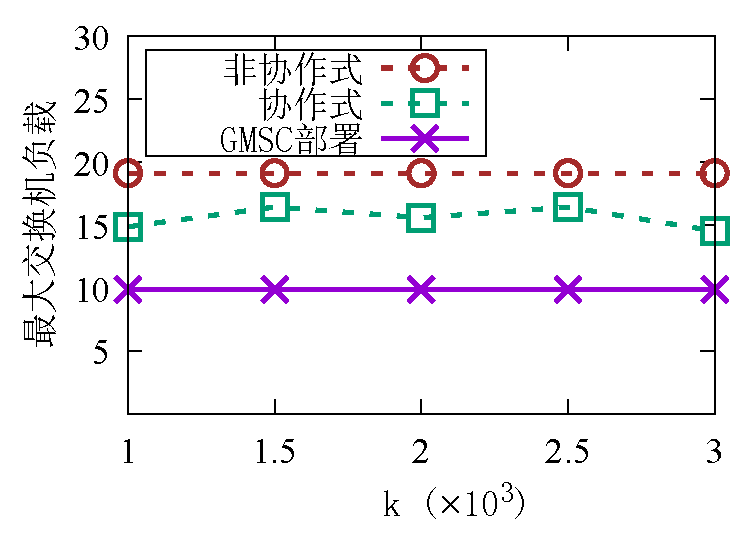
\includegraphics[width=\linewidth]{fig/msc_k_time.pdf}
		\caption{\textnormal{最大交换机负载与$k$,200000条流。}}
		\label{fig:msc,time,k}
		%\end{figure}
	\end{minipage}\vspace{-0.6em}\hspace{0.4em}
	\begin{minipage}[t]{0.48\linewidth}
		\centering
		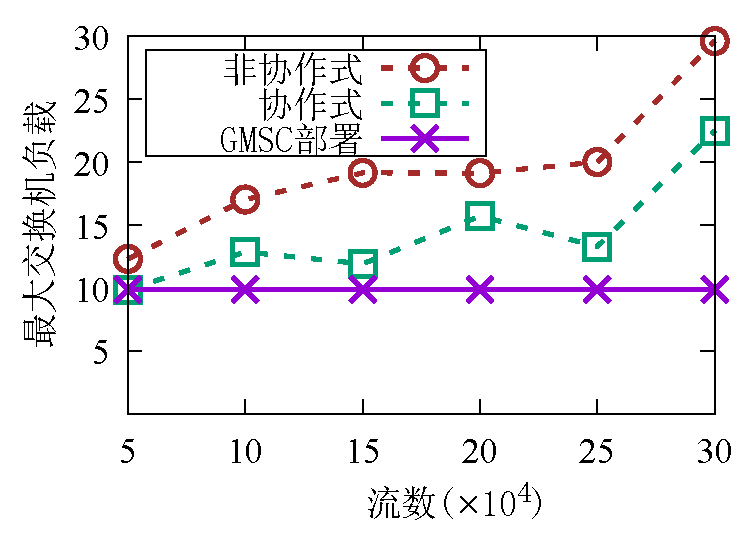
\includegraphics[width=\linewidth]{fig/msc_f_time.pdf}
		\caption{\textnormal{最大交换机负载与流数,$k=1000$。}}
		\label{fig:msc,time,flow}
	\end{minipage}\vspace{-0.6em}
\end{figure}

图\ref{fig:msc,err,k}和图\ref{fig:msc,err,flow}描述了交换机的最大负载。
由于交换机负载上限的限制,GMSC方法的最大交换机负载始终保持不变;
而协作式和非协作式的计算负载随着流数的增加明显上升,并且协作式CountMax由于引入了随机因素,导致最大交换机负载变得更加不易预测,体现在图中为较大的波动。



\section{小结}

本章首先建模分析了流量测量的分布式部署,从而提出了MSC问题并形式化定义。随后提出了GMSC算法并对其进行了分析。
最后通过仿真测试证明了GMSC的部署对CountMax的帮助。
\chapter{CountMax与GMSC的结合}
本章将在仿真环境中应用GMSC算法对CountMax进行部署,并评测其性能。
\section{测试指标与基准}
本章中用到的测试指标为平均估计误差和交换机上的最大处理数据包数。
其中平均估计误差的定义与第\ref{subsec:metric}节相同。
最大处理数据包数是统计每个交换机所处理的数据包的数量,取其最大值作为指标。
测试基准有两种,第一种是协作式CountMax,另一种是非协作式CountMax。
其中非协作式CountMax是在所有接入层交换机上都部署CountMax,并且处理所有经过的数据包。

对于一条流被多次测量的情况,采取多个测量值的平均值作为结果。

\section{测试结果}

\chapter{总结}
本章对本文的研究内容做一个总结。首先讨论GMSC与CountMax结合的可行性,随后介绍了本文解决的问题和未解决的问题。

\section{GMSC与CountMax的结合}

为了使得GMSC与sketch能够在现有的生产环境中应用,本节简要讨论GMSC在实际的SDN环境中实现的可行性。

GMSC的实现包括两个重要部分:其一是控制器与交换机之间的通信,其二是交换机上对数据包和掩码的匹配。
P4\cite{bosshart2014p4}是一种可行的一揽子解决方案。
P4是一个用来描述数据包处理流程的高级语言,它可以理解为是OpenFlow的升级版,是一种可编程的SDN南向协议。
Juniper已于2018年2月表示将支持P4作为控制器与交换机间的可选协议\cite{juniper2018p4}。
在UnivMon\cite{liu2016one}的实现部分中,数据平面中的采样、sketch等处理就是使用P4实现的。

\begin{figure}[ht]
	\centering
	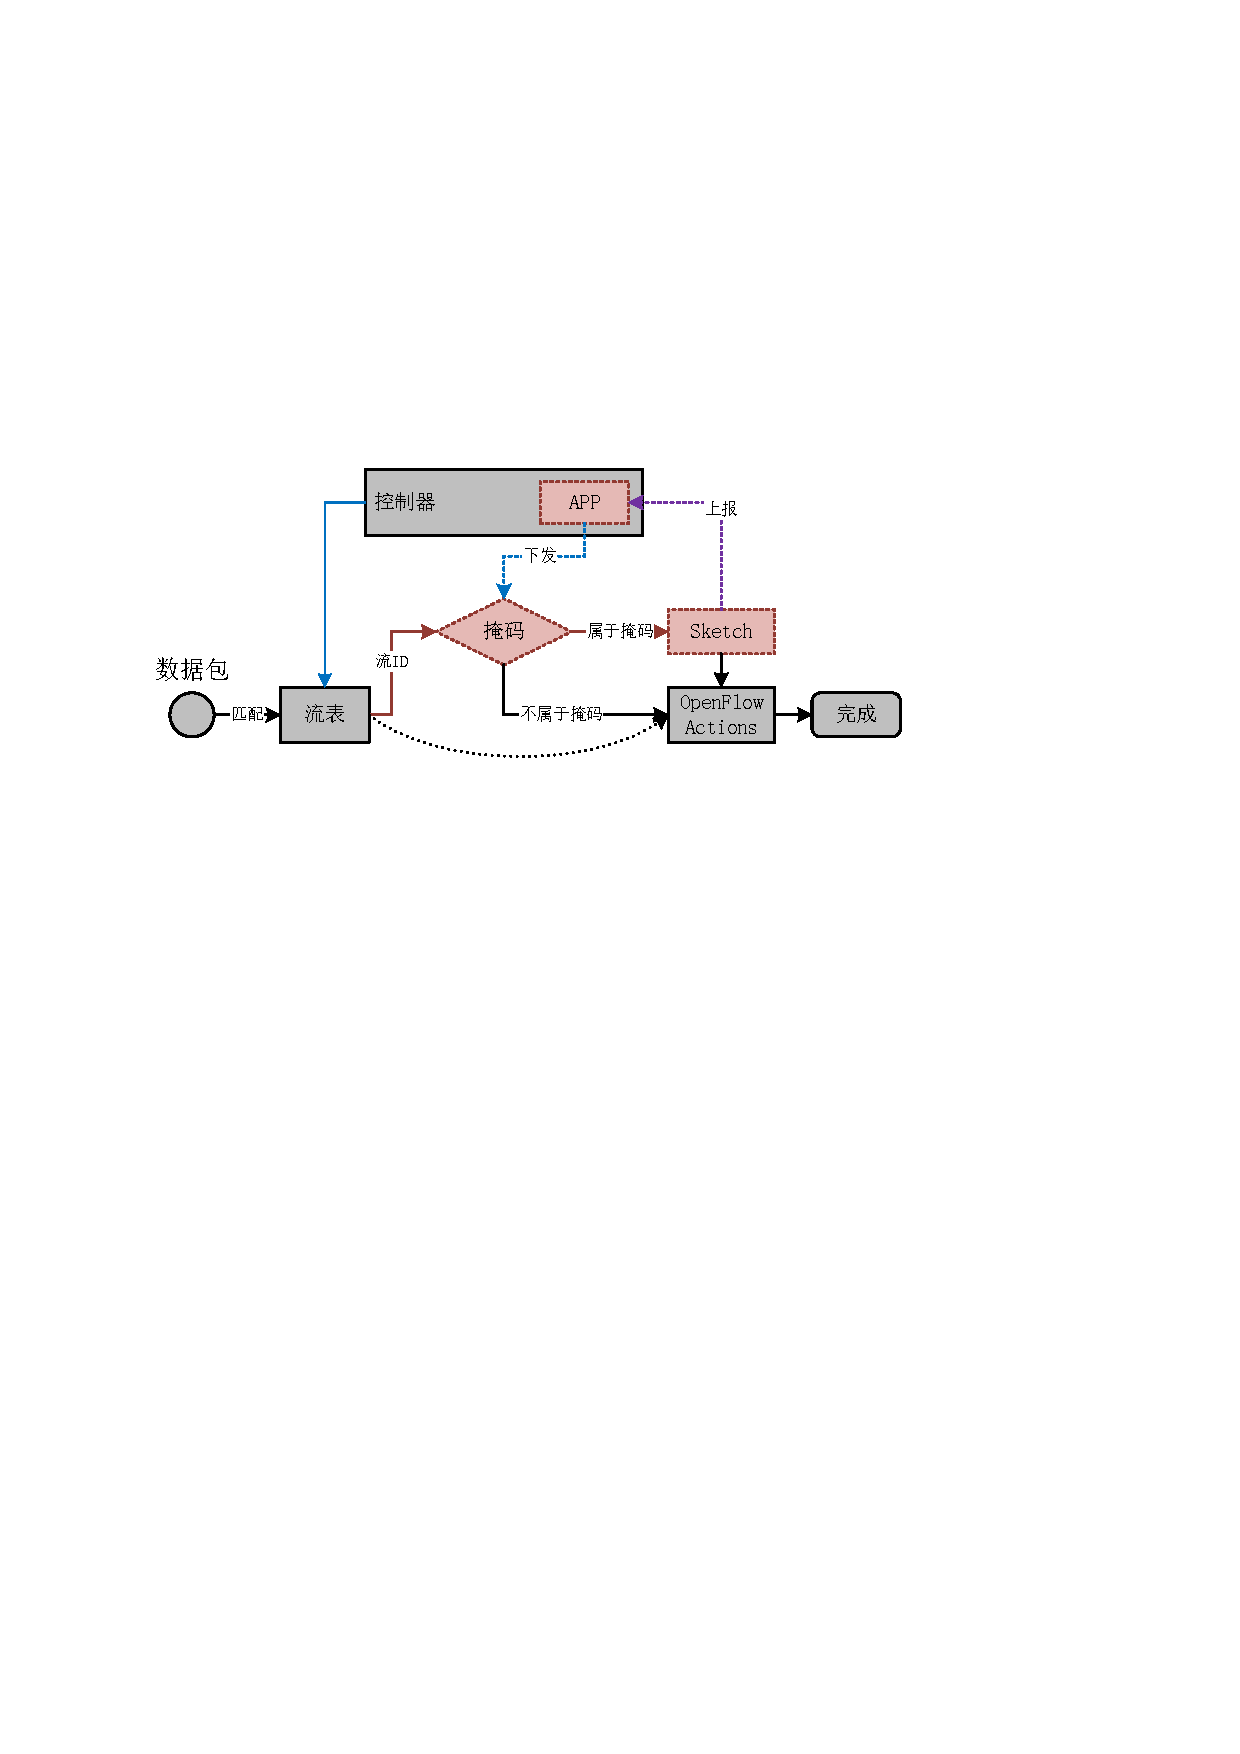
\includegraphics[width=0.75\textwidth]{fig/private.pdf}
	\caption{使用私有协议的实现方式}
	\label{fig:private}
\end{figure}

除P4外,对于可编程的交换机,我们还可以通过实现私有协议或者修改OpenFlow协议实现。
如UnivMon\cite{liu2016one}中控制器和交换机的通信就是通过私有的RPC(远程过程调用)管道实现的,本文第\ref{sec:proto}节中sketch数据的上报则是使用了专用的TCP端口。
如使用私有协议,可以在sketch运行的第一步添加判断流ID是否属于激活的掩码的判断,从而实现数据包和掩码的匹配。

图\ref{fig:private}为本文基于OVS平台上的私有协议的实现。其中红色框体属于本文开发的内容。
如图所示,在控制平面中,Sketch的控制APP寄宿在控制器中,通过独立的信道进行掩码的下发和流量统计数据的收集。
在数据平面中,所有的数据包在进行流表项匹配后,都会进行判断是否属于下发的掩码。
若属于,则交给sketch进行处理,随后再执行流表项中规定的操作。

修改OpenFlow协议的方法则是在正常的OpenFlow协议的基础上增加一种操作(Action),从而能够将“匹配掩码的数据包传输给sketch处理”的规则转换为流表直接发送到交换机。
在交换机上对这种自定义操作进行实现,使得它在被执行的时候会调用sketch处理此数据包。

\begin{figure}[ht]
	\centering
	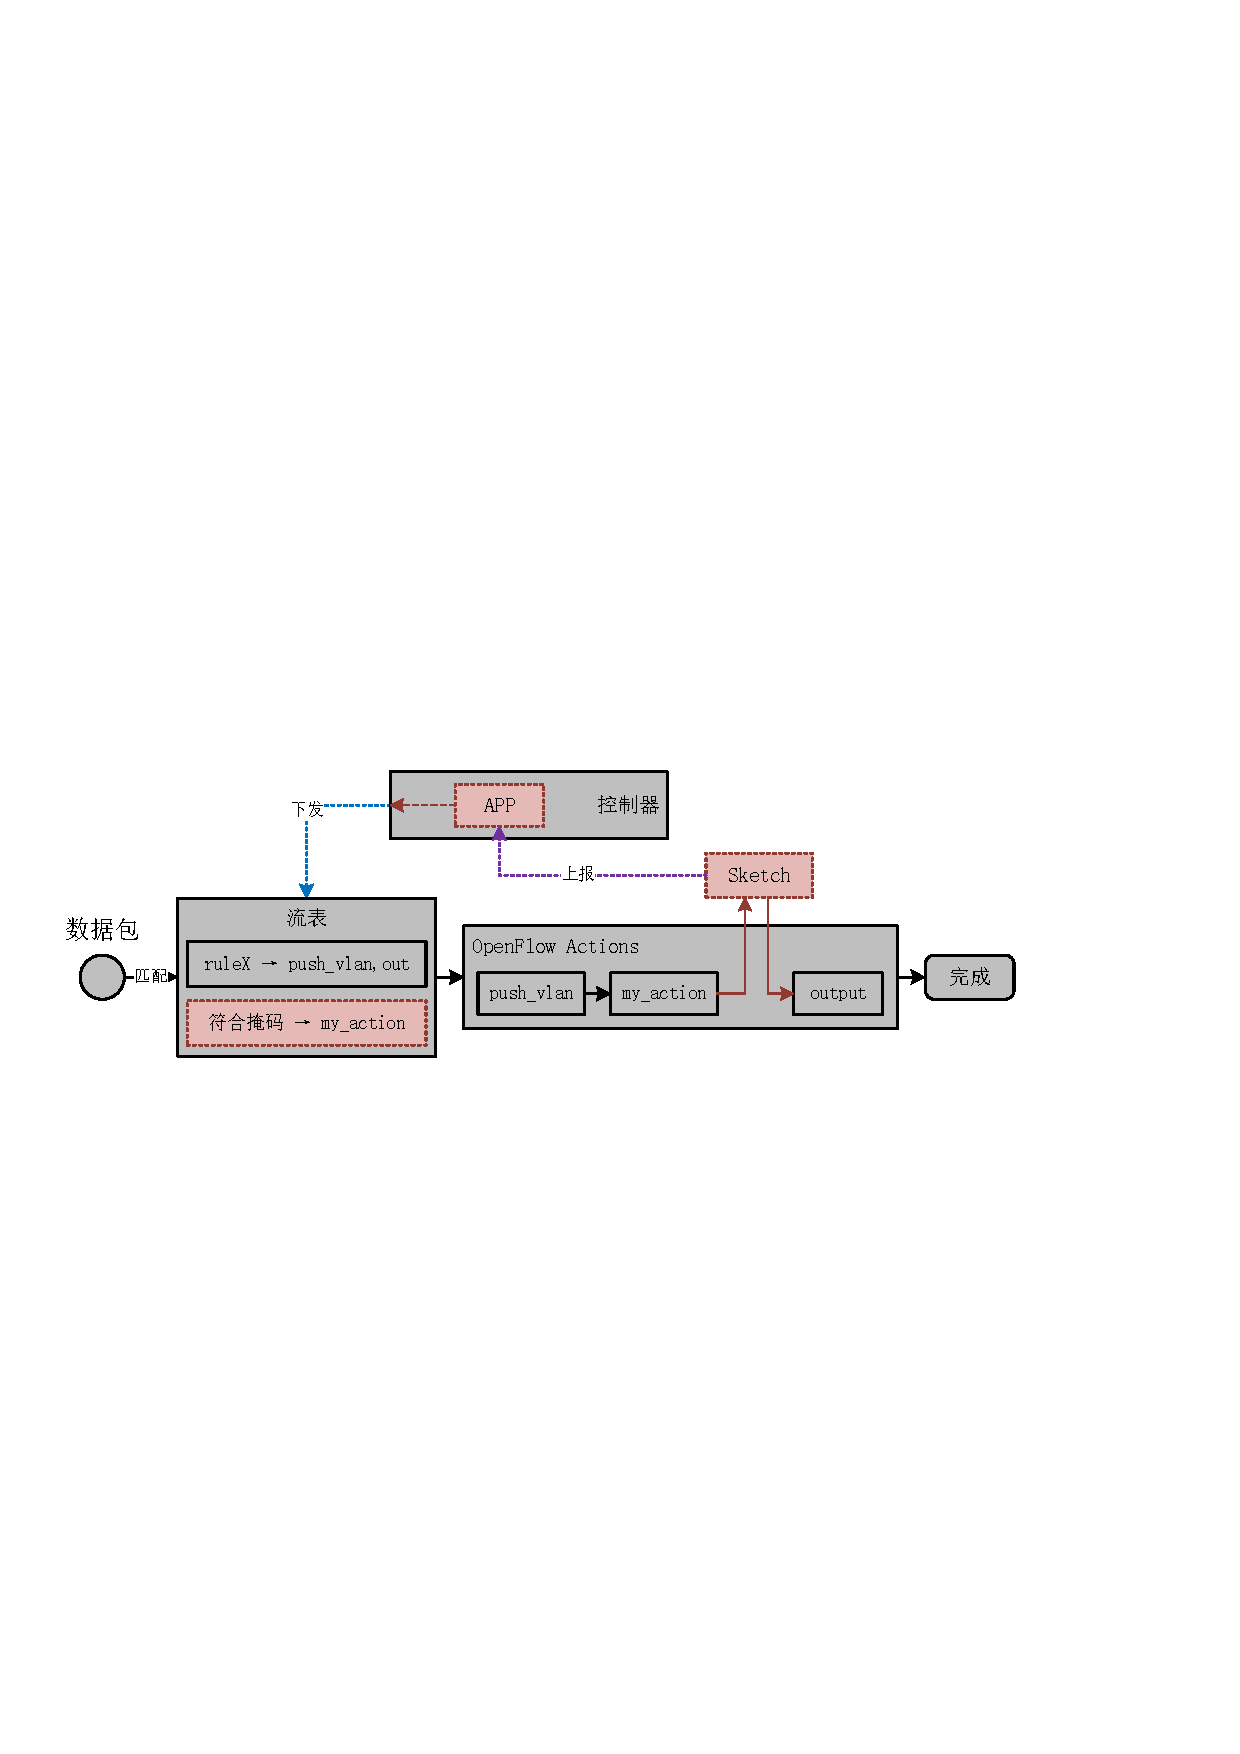
\includegraphics[width=\textwidth]{fig/ofaction.pdf}
	\caption{扩展OpenFlow的实现方式}
	\label{fig:ofaction}
\end{figure}

图\ref{fig:ofaction}为扩展OpenFlow协议实现方式的示意图。
首先编辑控制器和交换机上OpenFlow协议的实现,增加一个名为my\_action的操作,
并在交换机上将my\_action操作实现为调用sketch对数据包进行处理的操作。
控制APP通过控制器向交换机下发掩码的规则,指定匹配掩码的流要执行操作my\_action。
对于匹配的数据包,在交换机按照OpenFlow协议执行操作链时,my\_action会被执行,调用sketch进行统计,然后回到OpenFlow Action的管线中。

本文实现了以下功能:私有协议下的控制APP和OVS组件,以及扩展了OpenFlow、可通过控制台输入自定义操作的OVS。

\section{论文解决的问题}
本文首先梳理了软件定义网络中流量测量的重要性、调研并介绍了若干种现有的测量方法和sketch,且提出了流量测量分布式部署的问题。
随后,本文提出了名为CountMax的sketch。和现有的sketch相比,CountMax处理数据包所需的计算资源降低了约三分之一,但精度丝毫不逊色。
通过仿真模拟和系统集成测试,我们得出结论,CountMax可以胜任流量测量的任务。
之后,通过对流量测量分布式部署的建模与分析,本文引出了最大化流统计覆盖(MSC)问题,并给出了解决此问题的算法GMSC。
仿真模拟显示,将GMSC和CountMax结合,可以在有效地均摊计算负载的同时,提高测量精度。
最后,本文讨论了GMSC+CountMax在实际系统中的实现方法。

\section{尚未解决的问题}
本文尚未解决的问题,以及未来的研究方向主要有两点。
第一点是GMSC算法非常依赖流的先验知识。
对sketch进行预先部署不可避免的要依赖于先验知识,尽可能地减少所需的先验知识是一个研究方向。
另外,如果能够开发出可以动态调节的部署方式,利用实时数据动态进行部署也是一个可行的方向。
第二点是GMSC+CountMax系统的完善实现。本文中的系统实现只是验证可行性的原型,要让系统变得能够实际应用,还需要庞大的工程。
若采用私有协议,则必须考虑协议未来升级的可能性,注重可扩展性和兼容性。
若选择扩展OpenFlow协议,由于不同设备有着不同的OpenFlow实现,需要进行大量的设备适配和兼容性测试。
\bibliography{bib/ustc}

\appendix

\backmatter
%!TEX root = ../main.tex

\begin{acknowledgements}

在研究学习期间,我有幸得到了三位老师的教导,
他们是:我的导师,中国科大XXX研究员,中科院X昆明动物所马老师以及美国犹他大学的XXX老师。
三位深厚的学术功底,严谨的工作态度和敏锐的科学洞察力使我受益良多。
衷心感谢他们多年来给予我的悉心教导和热情帮助。

感谢XXX老师在实验方面的指导以及教授的帮助。
科大的XXX同学和XXX同学参与了部分试验工作,在此深表谢意。

\end{acknowledgements}

%!TEX root = ../main.tex

\begin{publications}

\section*{已发表论文}

\begin{enumerate}
\item \textbf{YU X}, XU H, YAO D, et al. Countmax: A lightweight and cooperative sketch measurement for software-defined networks[J]. IEEE/ACM Transactions on Networking (TON), 2018, 26(6):2774-2786. (CCF A类)
\item WANG H, \textbf{YU X}, XU H, et al. Integrating coflow and circuit scheduling for optical networks[J]. IEEE Transactions on Parallel and Distributed Systems, 2018. (CCF A类)
\end{enumerate}

\section*{已投稿论文}

\begin{enumerate}
\item XU H, YANG X, \textbf{YU X}, QIAN C, HUANG H. Maximum Flow Statistics Collection with Per-Switch Cost Constraint in SDNs[C]. IEEE/ACM International Symposium on Quality of Service, 2019.
\end{enumerate}
\end{publications}


\end{document}
